\chapter{Redes}
\section{Introducción, OSI vs TCP/IP}
Durante la asignatura de redes estudiamos el modelo OSI, sin embargo durante ésta asignatura nos centraremos en el estudio del modelo TCP/IP.\\

El modelo de Internet (TCP/IP) fue desarrollado en 1972 por el Departamento de Defensa de los Estados Unidos como una solución a un problema práctico de ingeniería.
\begin{figure}[H]
    \centering
    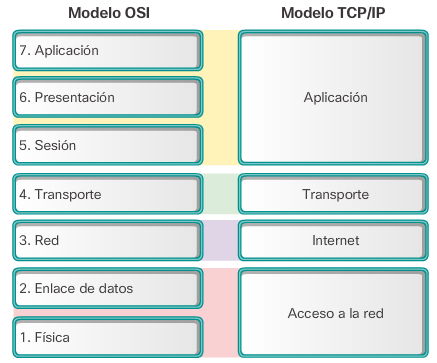
\includegraphics{img/OSIvsTCPIP.png}
    \caption{Comparativa de las capas de los modelos}
\end{figure}

En cambio, el modelo OSI(Open System Interconnection) fue propuesto como una solución teórica a los problemas de incompatibilidad entre redes.\\

Hoy en día es el modelo TCP/IP el que realmente se usa.
\section{Protocolo IPv4}
\begin{figure}[H]
    \centering 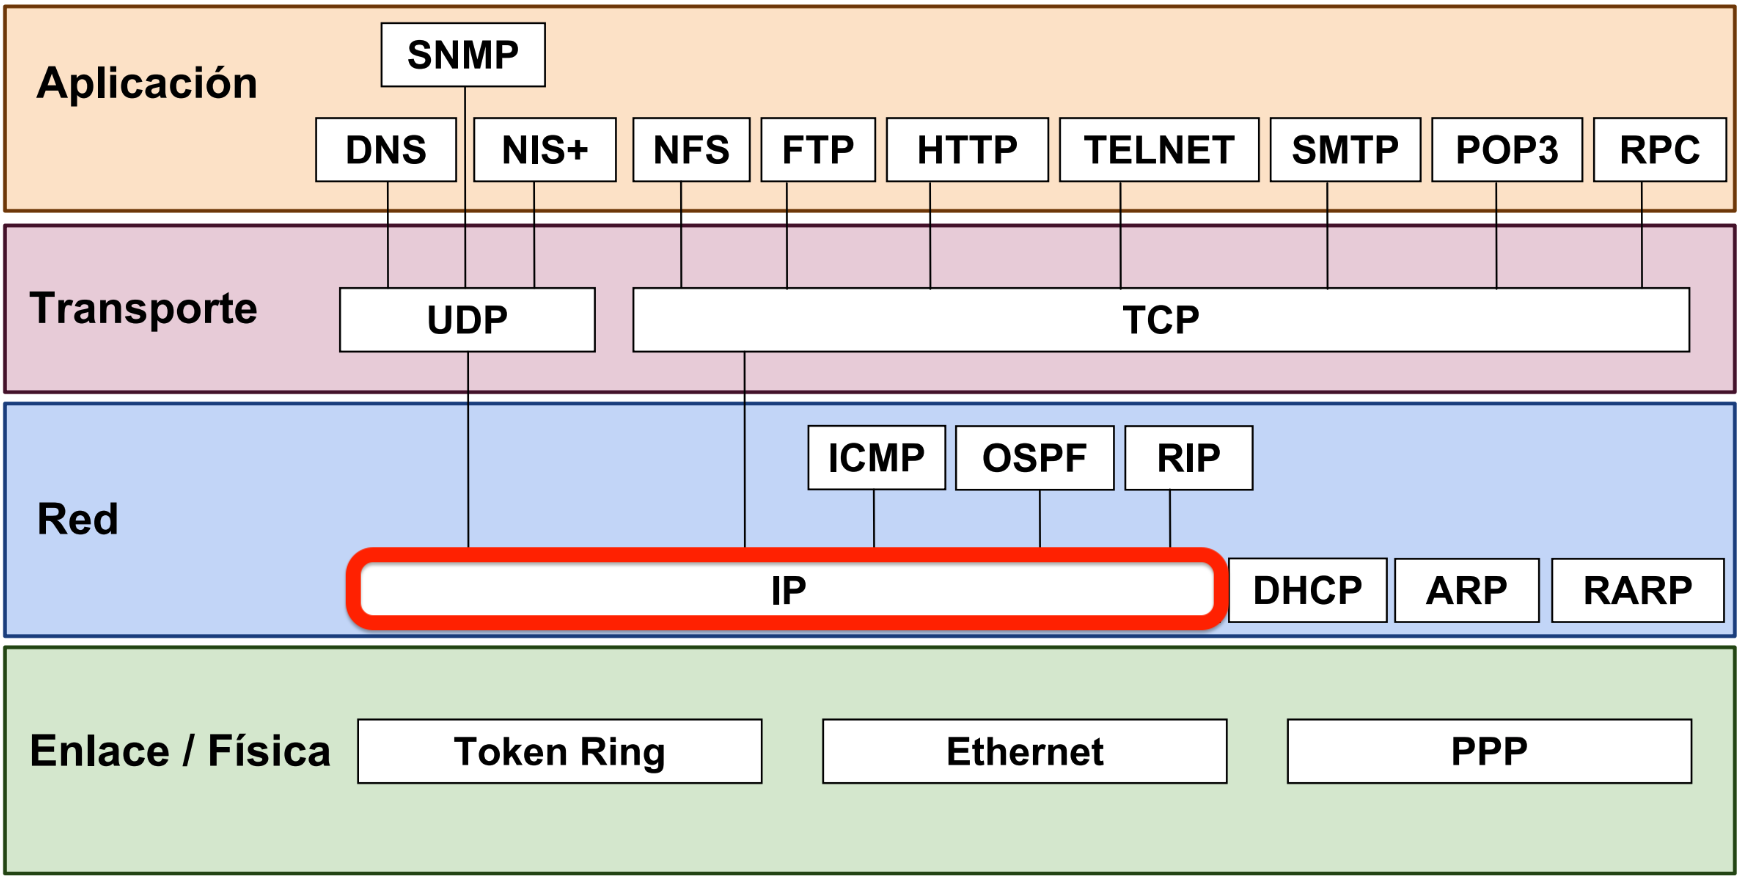
\includegraphics[width=0.7\textwidth]{img/IP.png}
\end{figure}
IP (Internet Protocol) es un protocolo de comunicación de datos digitales que transfiere paquetes a través de distintas redes físicas. Sus funciones básicas son:
\begin{itemize}
\item Encaminamiento: Saber por dónde tiene que enviar un mensaje.
\item Direccionamiento: Cómo nombrar las máquinas que están dentro de la red.
\item Fragmentación y Reensamblado: Traducir las tramas entre tecnologías distintas.
\end{itemize}
El protocolo IP es no orientado a conexión y no fiable, ésto quiere decir:
\begin{itemize}
    \item No detecta paquetes erróneos.
    \item No recupera paquetes perdidos.
    \item No garantiza que los paquetes lleguen en orden.
    \item No garantiza la detección de paquetes duplicados.
\end{itemize}
\subsection{Formato del mensaje IP}

El datagrama IP está formado por una cabecera IP seguida de un campo de datos. La cabecera para IPv4 es de la siguiente manera.

\begin{figure}[h]
\centering
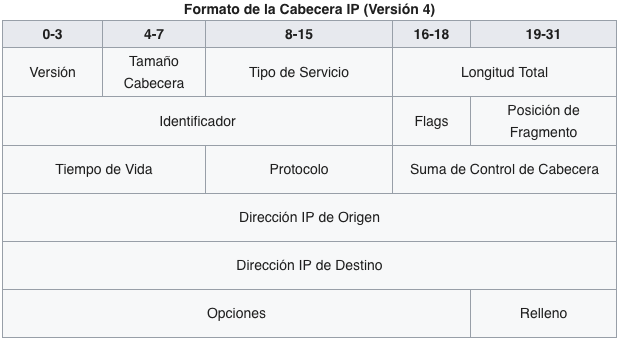
\includegraphics[width=0.85\textwidth]{img/datagramaIPv4.png}
\end{figure}

El campo opciones puede indicar:
\begin{itemize}
\item Encaminamiento desde el origen: lista de los encaminadores hasta llegar al destino. Usado para depuración o para saturar redes.
\item Registro de ruta: Cuando el datagrama llega al destinatario, tiene una lista de todos los routers por los que ha pasado.
\item Salto de tiempo: Cada router pone una marca de tiempo, se usa para medir el rendimiento de la red.
\end{itemize}

\subsection{Direccionamiento}

Una dirección IP es un número que identifica a una Interfaz en red  de un dispositivo que utilice el protocolo IP. La dirección IP no debe confundirse con la dirección MAC, que es un identificador de 48 bits para identificar de forma única la tarjeta de red y no depende del protocolo de conexión utilizando la red.\\

Las direcciones IPv4 se expresan mediante un número binario de 32 bits y se suelen expresar como números de notación decimal: se dividen los 32 bits de la dirección en cuatro octetos. El valor decimal de cada octeto está comprendido en el intervalo de 0 a 255. Ejemplo: [10.128.1.253]\\

\textbf{Tipos de direcciones IP.}\\
Las direcciones se dividen en dos campos de longitud variable: NetID (que identifica la red) y HostID (que identifica una máquina dentro de la red). Éstos rangos se indican mediante la máscara de red, que es un número que representa el número de bits de la NetID.

\begin{itemize}
\item Unicast: es el concepto más común en IP, se utiliza para un sólo dispositivo. [ej. 147.96.2.4]
\item Multicast: se utiliza para un grupo de receptores interesados. Se pueden utilizar direcciones comprendidas entre 224.0.0.0 - 239.255.255.255. [ej. 239.5.27.2]
\item Broadcast
	\begin{itemize}
	\item Limitada: usada para enviar a todas las máquinas de mi red LAN. [ej. 255.255.255.255]
    \item Dirigida: usada para enviar a todas las máquinas de una determinada red. [ej. 147.96.255.255]
	\end{itemize}
\item Anycast: envía el datagrama a la máquina más cercana de un grupo.
\end{itemize}

La direción IP debe ser única. Es la organización IANA quien se encarga de asignar las direcciones IP. Inicialmente se organizaron las direcciones IP en clases.

\begin{figure}[h]
\centering
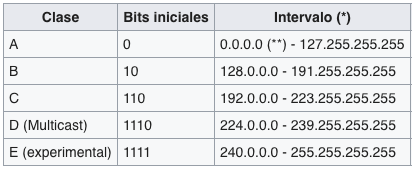
\includegraphics[width=0.65\textwidth]{img/clasesIP.png}
\end{figure}

El principal problema de esta forma de organización es el desperdicio de direcciones, por ello actualmente se utiliza una organización sin clases (CIDR).
\subsubsection{CIDR}
Classless Interdomain Routing, permite un uso más eficiente de las direcciones IP mediante la utilización de bloques de tamaños arbitrarios.\\

La notación CIDR permite expresar fácilmente las direcciones IP:\\

Consta de una direccion IPv4 de 32 bits seguida de una barra y un número, que indica el número de bits que identifican al bloque.\\

{\centering
    \textbf{122.233.2.1/24}\\
}


Ésta dirección indica que los primeros 24 bits de la dirección son los que identifican al bloque (Prefijo de red), y los otros 8 menos significativos son los que identifican al host.\\
\subsubsection{Direcciones reservadas}
El \textbf{identificador de host} tiene dos excepciones, según el valor de sus bits:
\begin{enumerate}
    \item \textbf{Todo a ceros:} indica que se trata de la dirección que identifica a la red (no de ninguna máquina), por tanto nunca se puede utilizar como dirección de destino.
    \item \textbf{Todo a unos:} indica que se trata de una dirección de broadcast, y al usarse como dirección de destino enviará el paquete a todas las máquinas de la red local.
\end{enumerate}
A parte, existen otras direcciones reservadas:
\begin{itemize}
  \item \textbf{10.x.x.x} red privada de clase A.
  \item \textbf{172.16.0.0 - 172.31.255.255} son 16 redes privadas de clase B.
  \item \textbf{192.168.x.x} son 256 redes privadas de clase C
  \item \textbf{127.x.x.x} Direcciones de Loopback (reenvían los paquetes a la misma máquina)
  \item \textbf{224.0.0.xxx} son direcciones multicast reservadas, por ejemplo:
  \begin{itemize}
      \item \textbf{224.0.0.1} Todos los hosts.
      \item \textbf{224.0.0.2} Todos los routers.
  \end{itemize}
\end{itemize}

%ARP
\section{Protocolo ARP}
\begin{figure}[H]
    \centering
    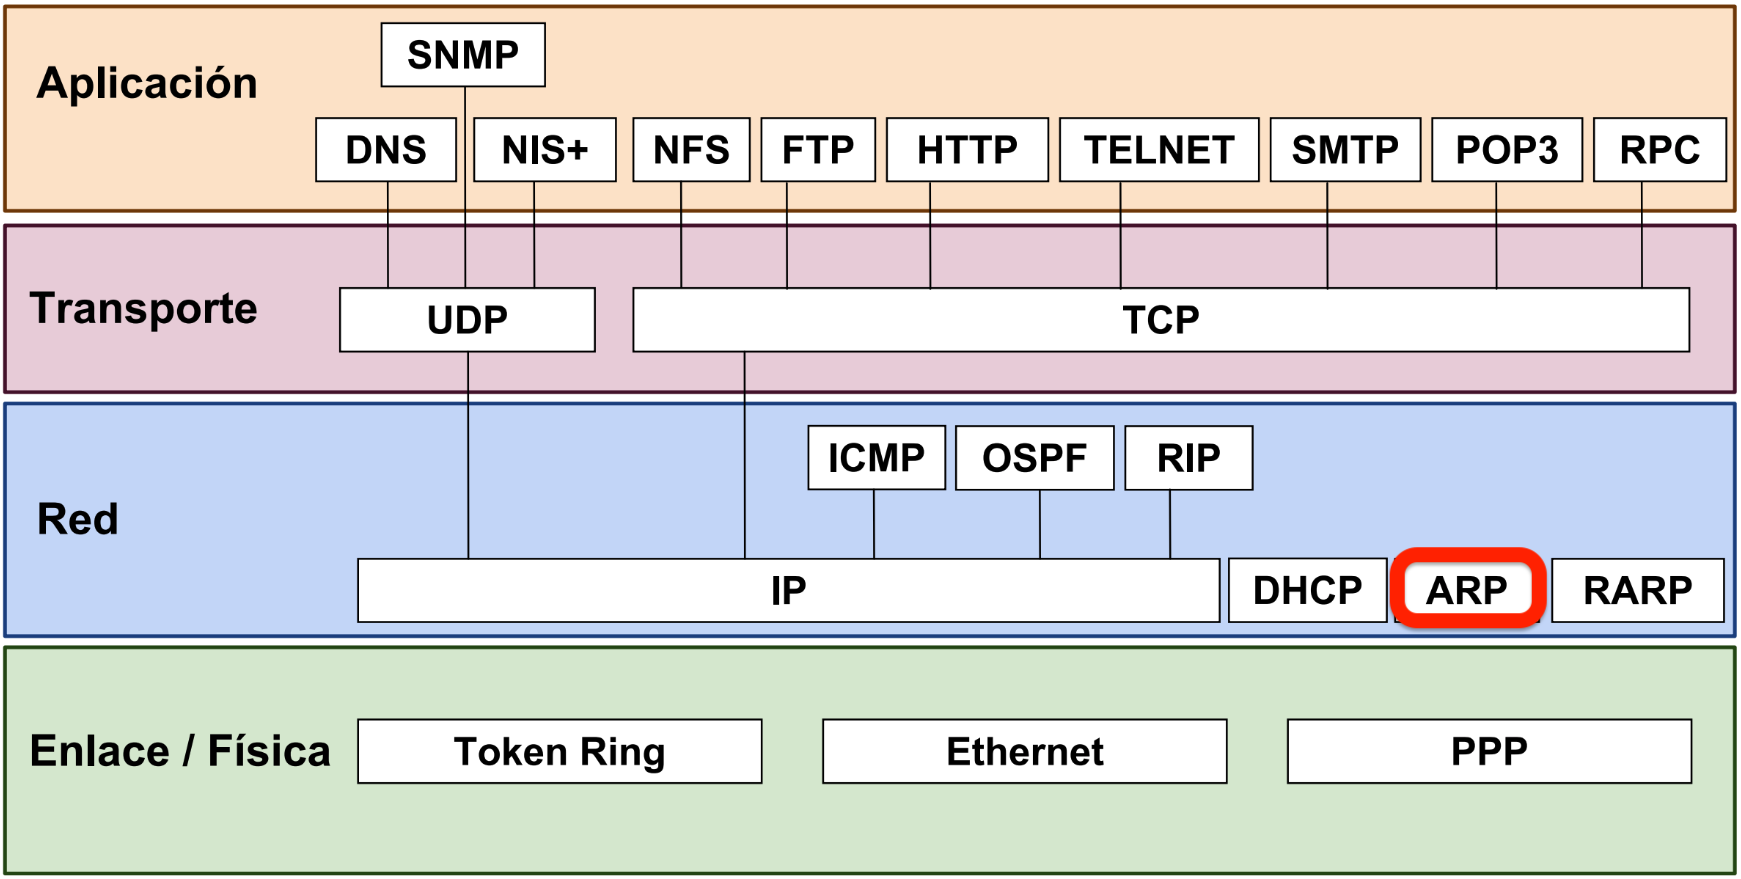
\includegraphics[width=0.7\textwidth]{img/ARP.png}
\end{figure}
\vspace{2cm}
Un datagrama IP tiene la siguiente forma.

\begin{table}[h] \centering \begin{tabular}{|c|c|}
\hline Cabecera IP & Datos \\ \hline \end{tabular}
\end{table}
A la hora de ser enviado, se encapsula \textbf{dentro del campo de datos} de otra trama más grande, la trama ARP.

\begin{table}[h] \centering \begin{tabular}{|l|c|c|l|l|}
\hline MAC Destino & MAC Origen & Protocolo & \textbf{Datos} & CRC \\ \hline \end{tabular}
\end{table}
\vspace{2cm}
ARP se encarga de encontrar la dirección MAC que corresponde a una determinada dirección IP. Para ello se envía un paquete (ARP request) a la dirección de difusión de la red (broadcast, MAC = FF FF FF FF FF FF) que contiene la dirección IP por la que se pregunta, y se espera a que esa máquina responda (ARP reply) con su dirección MAC.\\

Cada máquiena mantiene una tabla ARP en la que guarda las direcciones IP de las últimas máquinas con las que ha conectado, junto con su dirección MAC.
\newpage
%ICMP
\section{Protocolo ICMP}
\begin{figure}[H]
    \centering
    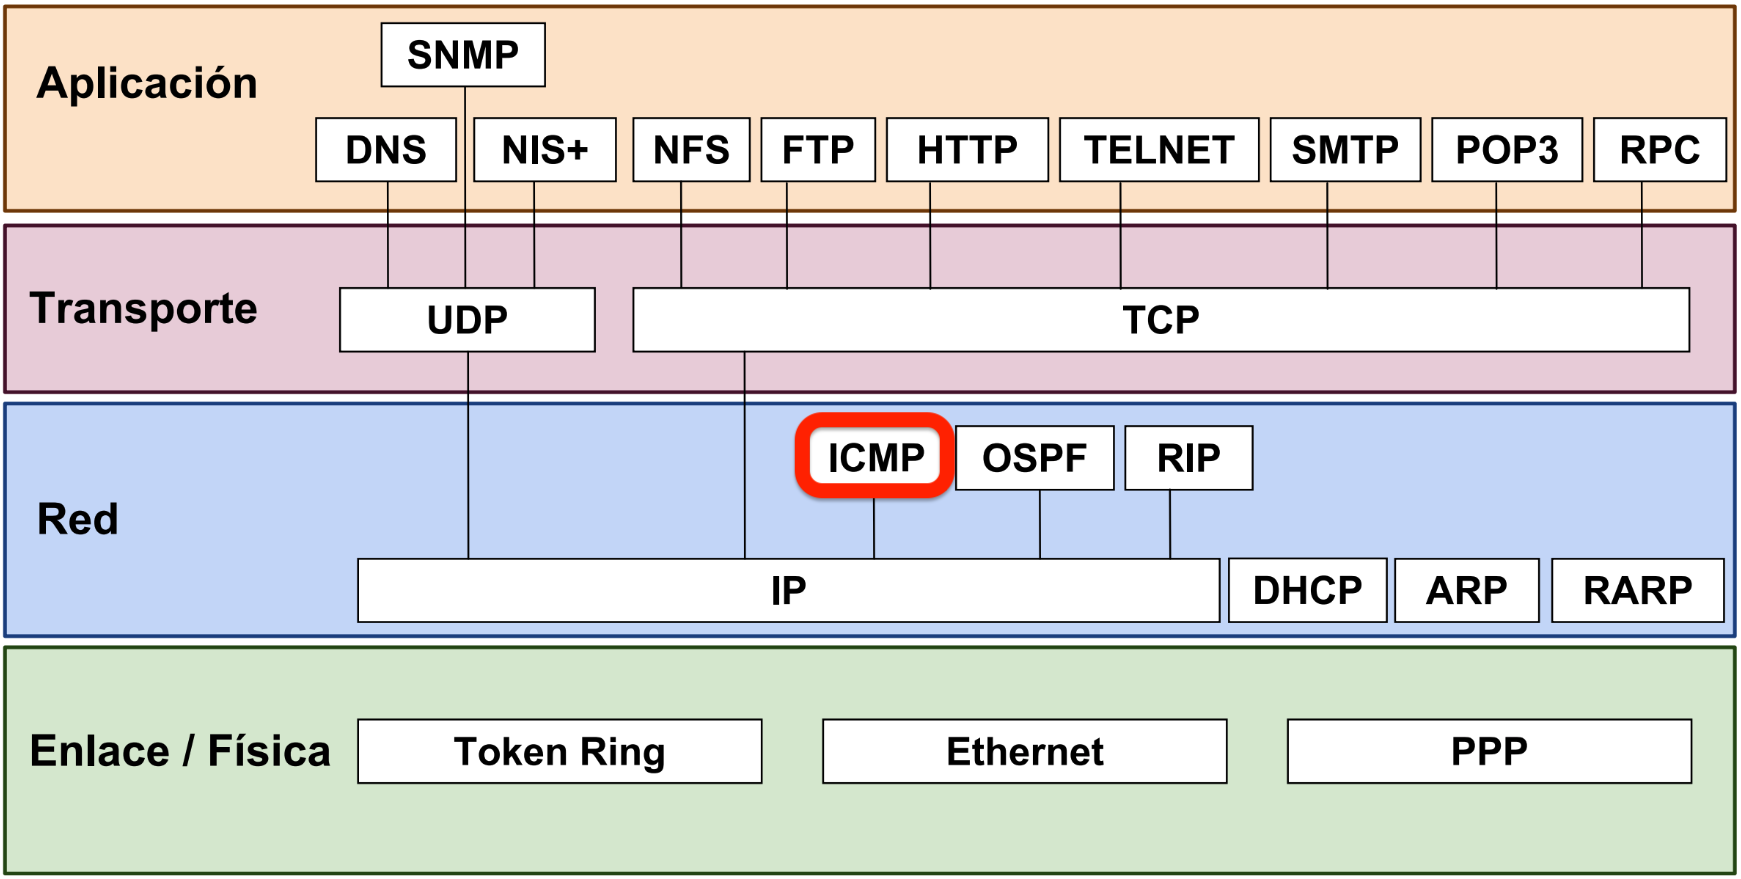
\includegraphics[width=0.7\textwidth]{img/ICMP.png}
\end{figure}
ICMP (Internet Control Message Protocol) es un protocolo de mensajes que viajan dentro del datagrama IP. Se usa para enviar mensajes de error, indicando por ejemplo que un router o host no puede ser localizado. También puede ser utilizado para transmitir mensajes de información.
\\\\
Algunos tipos de mensajes ICMP:
\begin{itemize}
\item De información
	\begin{itemize}
	\item \textbf{Echo Reply}
	\item \textbf{Echo Request}
    \item Redirect
    \item Router Solicitation
    \item Router Advertisement
	\end{itemize}
\item De error
	\begin{itemize}
	\item Destination Unreachable
    \item Source Quench
    \item Time Exceeded
    \item Parameter Problem
	\end{itemize}
\end{itemize}
\subsection{ECHO Request/Reply}
Como mensajes a destacar tenemos ECHO Request y ECHO Reply, que son los que utiliza la orden "ping" para comprobar la conexión.\\

Éstos mensajes tienen el siguiente formato:

\begin{table}[H]
\centering
\begin{tabular}{|c|c|c|}
\hline
\rowcolor[HTML]{9AFF99} 
Tipo = 0 & Código = 0  & Checksum \\ \hline
\rowcolor[HTML]{FDAAAA} 
\multicolumn{2}{|c|}{\cellcolor[HTML]{FDAAAA}{\color[HTML]{000000} Identificador}} & {\color[HTML]{000000} Número de secuencia} \\ \hline
\rowcolor[HTML]{FDAAAA} 
\multicolumn{3}{|c|}{\cellcolor[HTML]{FDAAAA}Datos :::}  \\ \hline
\end{tabular}
\end{table}
\begin{itemize}
    \item \textbf{Identificador:} Permitte establecer correspondencia entr solicitud (Request) y respuesta (Reply); ambos con el mismo identificador.
    \item \textbf{Secuencia:} También se utiliza para establecer la correspondencia entre solicitud y respuesta, cuando se envían varios Echo Requests consecutivos con el mismo identificador.
    \item \textbf{Datos:} Un número determinado de bytes aleatorios.
\end{itemize}

%DHCP
\begin{onepage}
\section{Protocolo DHCP}
\begin{figure}[H]
    \centering
    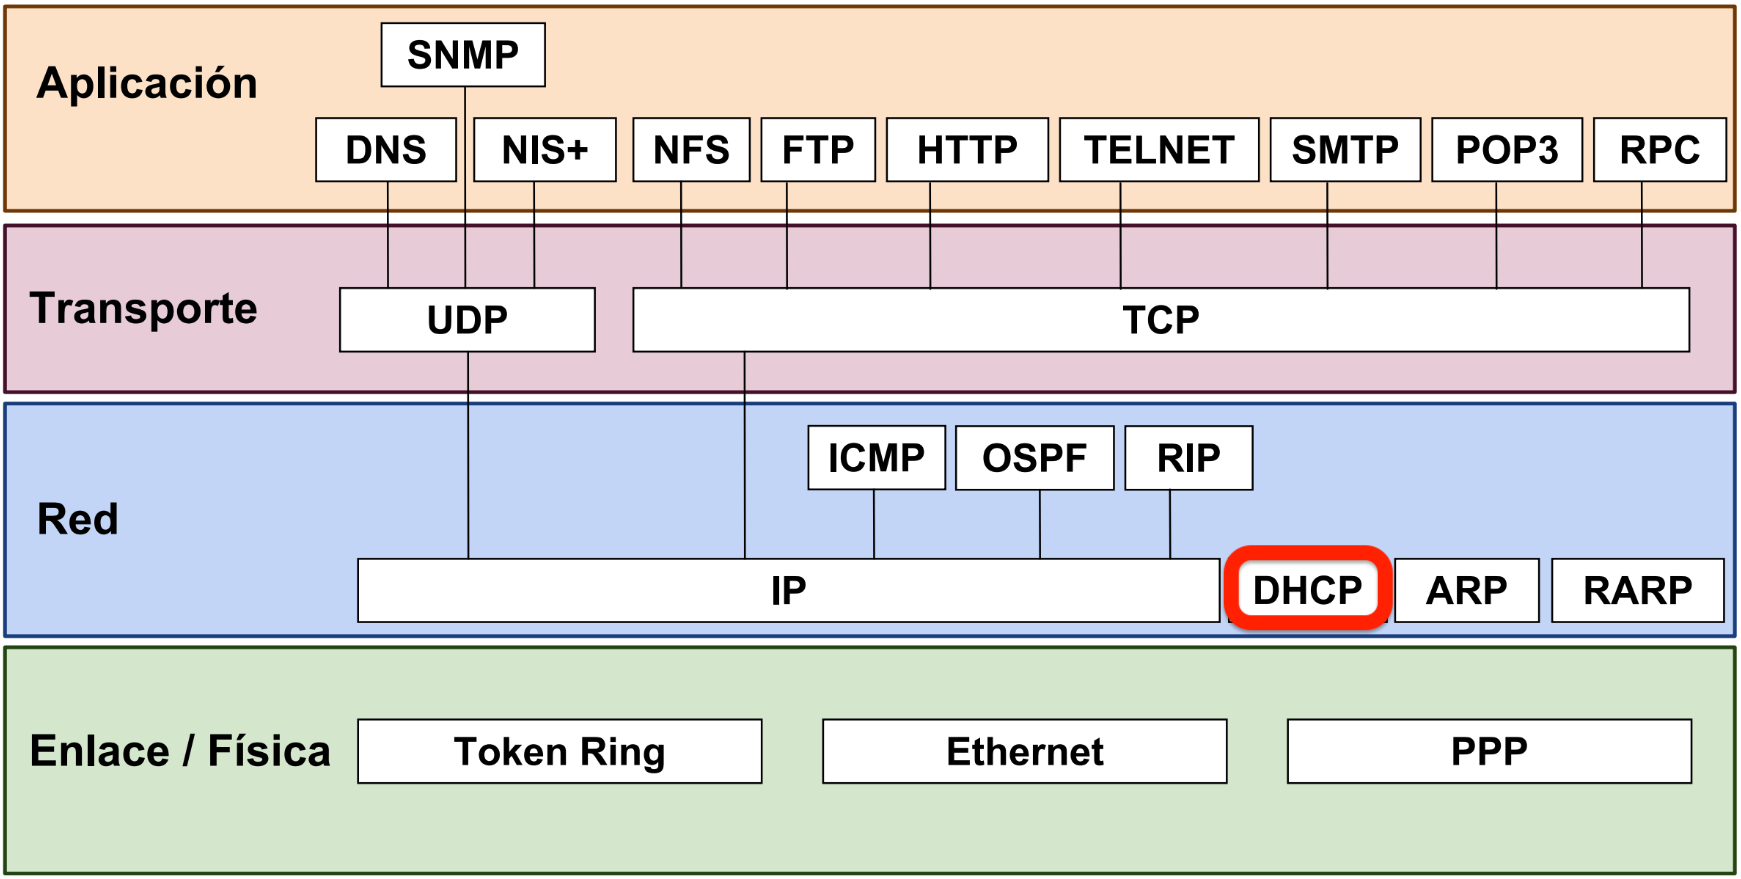
\includegraphics[width=0.7\textwidth]{img/DHCP.png}
\end{figure}

DHCP (Dynamic Host Configuration Protocol) es un protocolo que permite la configuración dinámica de direcciones IP y máscaras de red, router predeterminado, servidor DNS, y otros parámetros de configuración de red.\\

Este servidor posee una lista de direcciones IP dinámicas y las va asignando a los clientes conforme éstas van quedando libres, sabiendo en todo momento quién ha estado en posesión de esa IP, cuánto tiempo la ha tenido y a quién se la ha asignado después. Así los clientes de una red IP pueden conseguir sus parámetros de configuración automáticamente.\\

Algunas de sus \textbf{características} son:
\begin{itemize}
    \item Es un protocolo de red de tipo \textbf{cliente/servidor} sobre UDP en los puertos 67 (servidor) y 68
(cliente).
    \item Tiene un mecanismo de \textbf{control de errores} basado en sumas de comprobación, temporizadores y retransmisiones.
    \item Puede proveer de una servidor \textbf{TFTP} al dispositivo cliente. TFTP se utiliza para transferir pequeños archivos entre ordenadores en una red, como imágenes de arranque.
    \item En redes grandes con muchos enlaces, un servidor DHCP es ayudado por \textbf{DHCP relay agents} situados en routers intermedios. Estos agentes retransmiten los mensajes entre cliente y servidor situados en distintas subredes.
\end{itemize}
\end{onepage}
\subsection{Mensajes DHCP}
Estos son algunas de las operaciones que permite el protocolo.
\begin{itemize}
    \item DHCPDISCOVER: Mensaje del cliente (broadcast) para descubrir los servidores disponibles (puede contener la última dirección IP asignada).
    \item DHCPOFFER: Respuesta de los servidores, con una oferta de parámetros de configuración. Puede
    recibirse más de una.
    \item DHCPREQUEST: Petición de oferta del cliente (broadcast, para notificar a todos los servidores) o extensión del tiempo de cesión. El servidor seleccionado se especifica en una opción (Server Identifier, código 54).
    \item DHCPACK: Mensaje de confirmación (broadcast) y cierre desde el servidor hacia el cliente indicando los parámetros definitivos.
    \item DHCPRELEASE: Mensaje del cliente para informar al servidor de que ha finalizado el uso de
    la dirección IP.
\end{itemize}
\subsection{Datagrama DHCP}
\begin{figure}[H]
    \centering
    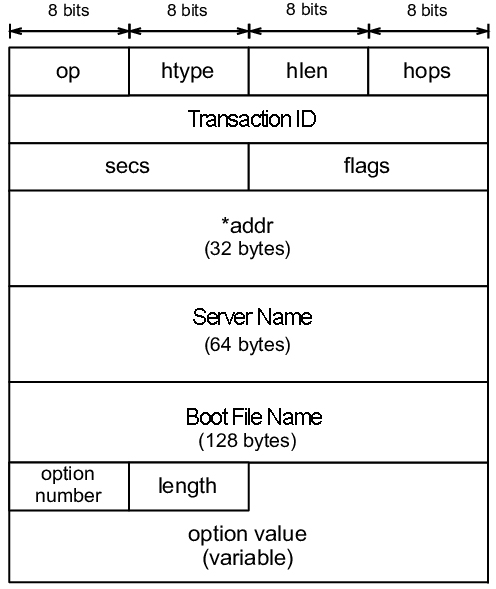
\includegraphics[width=0.5\textwidth]{img/DHCPformat.jpg}
    \caption{*addr: se guardan algunas direcciones como las de cliente y servidor.}
\end{figure}
%TCP
\newpage
\section{Protocolo TCP}
\begin{figure}[H]
    \centering
    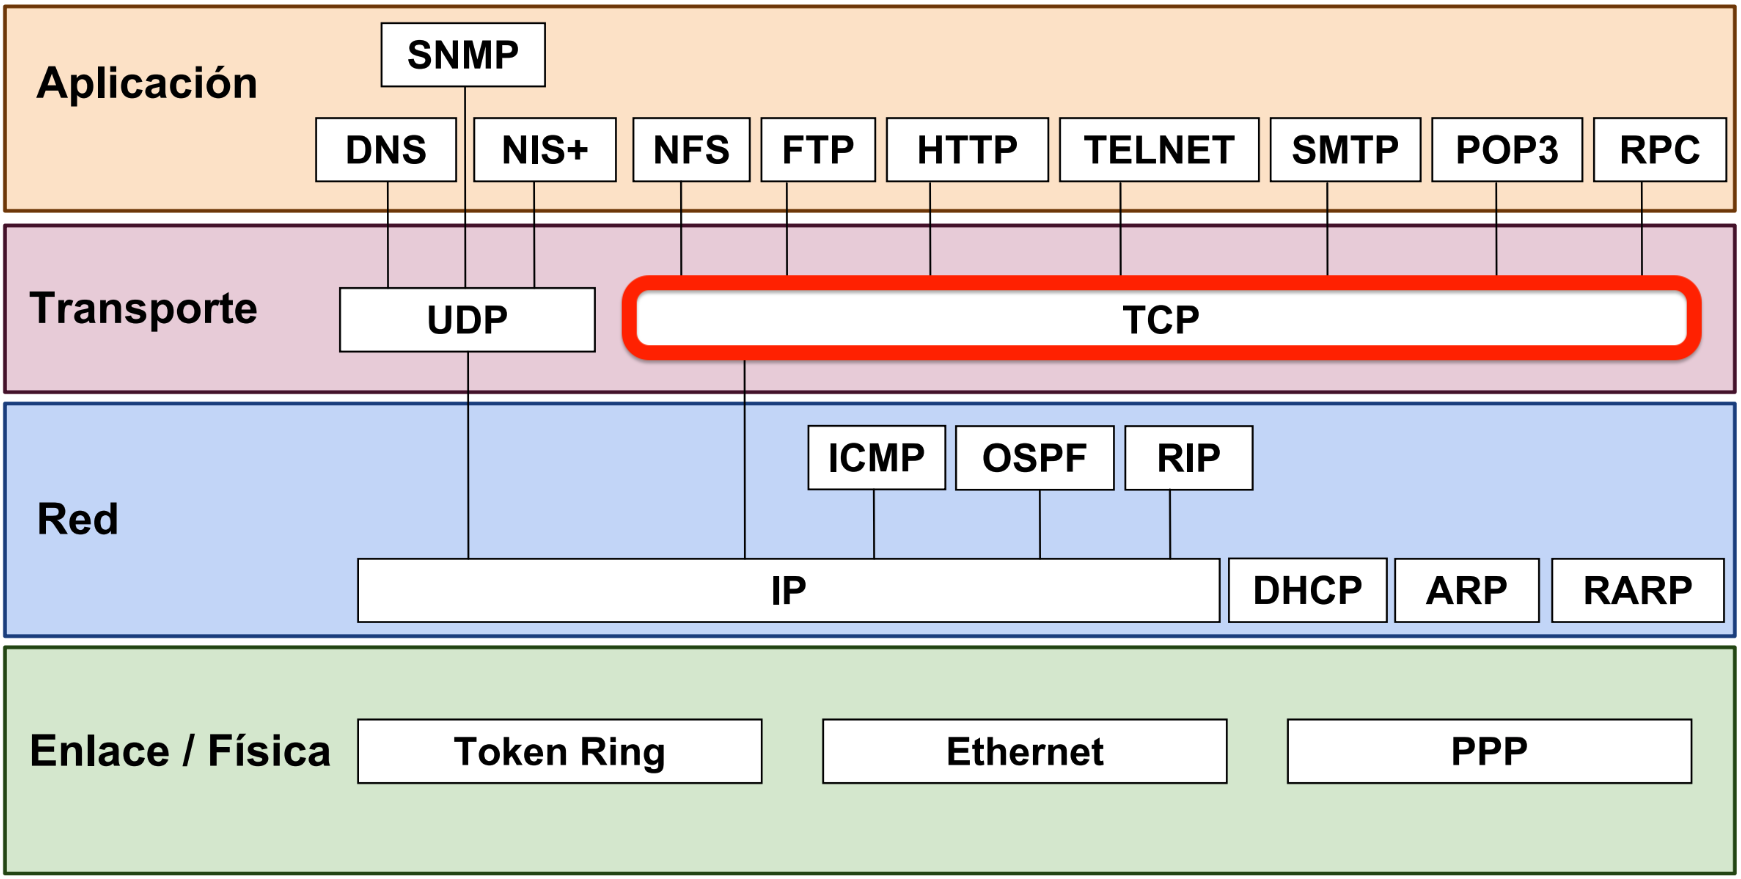
\includegraphics[width=0.7\textwidth]{img/TCP.png}
\end{figure}
TCP (Transmission Control Protocol) es un protocolo de transporte fiable y orientado a conexión (a diferencia de UDP, que es no fiable y no orientado a conexión). También proporciona un mecanismo para distinguir distintas aplicaciones dentro de una misma máquina, a través del concepto de puerto.

\subsubsection{Características de TCP}
\begin{itemize}
    \item Reordena los segmentos procedentes del protocolo IP y permite comenzar y finalizar la comunicación de forma consensuada entre ambas máquinas. \textbf{Orientado a conexión}.
    \item Monitorea el flujo de datos y así evita la saturación de la red. \textbf{Ventana Deslizante}.
    \item Permite que los datos se formen en segmentos de longitud variada para "entregarlos" al protocolo IP.
    \item Sirve para establecer la comunicación entre procesos de distintas máquinas. \textbf{Puertos}.
    \item Permite \textbf{multiplexar} los datos, es decir, que la información que viene de diferentes fuentes pueda circular simultáneamente por el mismo medio.
\end{itemize}
\subsection{Datagrama TCP}
\begin{figure}[H]
    \centering
    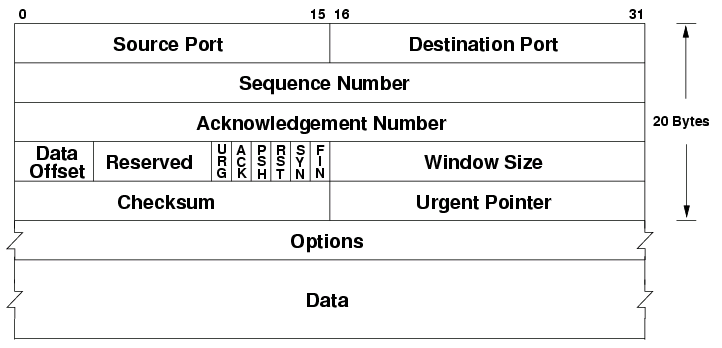
\includegraphics[width=0.85\textwidth]{img/TCPformat.png}
    \caption{Se divide en dos partes: datos (Data) y cabecera (Resto de campos).}
\end{figure}
\begin{itemize}
    \item \textbf{Source/Destination Port}: Identifican ambos extremos de la conexión.
    \item \textbf{Sequence/Acknowledgement Number}: Números de secuencia y confirmación expresados en bytes.
    \item \textbf{Reserved}: No se usa y se pone a 0.
    \item \textbf{Data offset}: Longitud de la cabecera.
    \item \textbf{Flags}
    \begin{itemize}
        \item URG: El segmento transporta datos urgentes (URG=1) desde el primer byte hasta el nº de byte especificado en el campo puntero urgente. TCP notifica a la aplicación de los datos urgentes (mediante la señal SIGURG), y ésta se encarga de tratarlos.
        \item ACK: El segmento contiene un número de confirmación válido (ACK=1). Todos los segmentos de una conexión TCP, excepto el primero, llevan ACK=1.
        \item PSH: Los datos deben ser entregados inmediatamente a la aplicación (PSH=1), o pueden almacenarse en el buffer (PSH=0).
        \item RST: Utilizado para abortar una conexión.
        \item SYN: Utilizado en el establecimiento de la conexión y sincronizar los números de
secuencia iniciales.
        \item FIN: Utilizado en la finalización de la conexión.
    \end{itemize}
    \item \textbf{Window Size}: Tamaño de la ventana.
    \item \textbf{Checksum}: Suma de comprobación.
    \item \textbf{Urgent Pointer}: Puntero que identifica el último byte de datos urgentes.
    \item \textbf{Options}: Campo de opciones de longitud variable.
    \item \textbf{Data}: Campo de datos de longitud variable.
\end{itemize}
\begin{onepage}

\subsection{Fases de conexión}
Ya sabemos que TCP es un protocolo orientado a conexión, ahora vamos a ver detenidamente como se comunican dos máquinas.
\subsubsection{Fase de Establecimiento}
\begin{figure}[H]
    \centering
    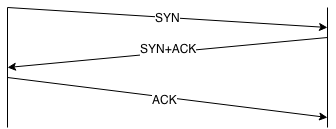
\includegraphics[width=0.55\textwidth]{img/SYN3.png}
\end{figure}
Una máquina (\textbf{servidor}) abre socket en un determinado puerto TCP y se queda a la escucha de nuevas conexiones (apertura pasiva).\\

Otra máquina (\textbf{cliente}) realiza una apertura activa de un puerto enviando un paquete SYN al servidor como parte de la negociación en tres pasos. En el lado del servidor se comprueba si el puerto está abierto, es decir, si existe algún proceso escuchando en ese puerto.\\

En caso de no estarlo, se envía al cliente un paquete de respuesta con el bit RST activado, lo que significa el rechazo del intento de conexión.\\

En caso de que sí se encuentre abierto el puerto, el lado servidor respondería a la petición SYN válida con un paquete SYN/ACK. Finalmente, el cliente debería responderle al servidor con un ACK, completando así la negociación en tres pasos (SYN, SYN/ACK y ACK) y la fase de establecimiento de conexión.\\

Es interesante notar que existe un número de secuencia generado por cada lado, ayudando de este modo a que no se puedan establecer conexiones falseadas (spoofing).\\

\begin{tcolorbox}[
title=SYN Flood,
colback=blue!5!white,
colframe=blue!75!black,
fonttitle=\bfseries]
Es una vulnerabilidad en el protocolo que consiste en enviar una gran cantidad de segmentos TCP con el flag SYN activado, saturando el servidor (ataque DoS), ya que asigna recursos a cada intento de conexión. Para evitarlos se puede:
\begin{itemize}
    \item Limitar el número de conexiones.
    \item Aceptar conexiones sólo de IP’s confiables.
    \item Retrasar la asignación de recursos usando SYN cookies.
\end{itemize}
\end{tcolorbox}
\end{onepage}
\subsubsection{Fase de Transferencia}
Durante la etapa de transferencia de datos, una serie de mecanismos claves determinan la fiabilidad y robustez del protocolo. Entre ellos están incluidos el uso del \textbf{número de secuencia} para ordenar los segmentos TCP recibidos y detectar paquetes duplicados, \textbf{checksums} para detectar errores, \textbf{temporizadores} para detectar pérdidas o retrasos y \textbf{ventanas deslizantes} para el control de flujo de datos.
\subsubsection{Fase de Finalización}
La fase de finalización puede realizarse de dos maneras:
\begin{itemize}
    \item \textbf{Finalización de 4 vías}:
\begin{figure}[H]
    \centering
    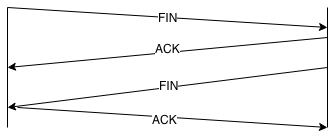
\includegraphics[width=0.55\textwidth]{img/FIN4.png}
\end{figure}
    \begin{enumerate}
        \item El cliente deja de enviar datos al servidor, y le envía un paquete con el flag FIN activado.
        \item El servidor le responde con un paquete con el flag ACK.
        \item Cuando el servidor deja de tener datos para enviar, envía otro paquete con el flag FIN.
        \item El cliente le responde con ACK, tras lo cual se cierra la conexión.
    \end{enumerate}
    \item \textbf{Finalización de 3 vías}:
\begin{figure}[H]
    \centering
    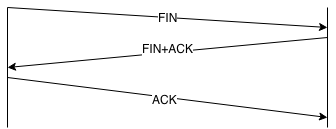
\includegraphics[width=0.55\textwidth]{img/FIN3.png}
\end{figure}
    \begin{enumerate}
        \item El cliente deja de enviar datos al servidor, y le envía un paquete con el flag FIN activado.
        \item El servidor le responde con un paquete con los flags FIN y ACK activados y deja de enviar datos.
        \item El cliente le responde con ACK, tras lo cual se cierra la conexión.
    \end{enumerate}

\end{itemize}
\subsubsection{Diagrama de estados}
\begin{figure}[H]
    \centering
    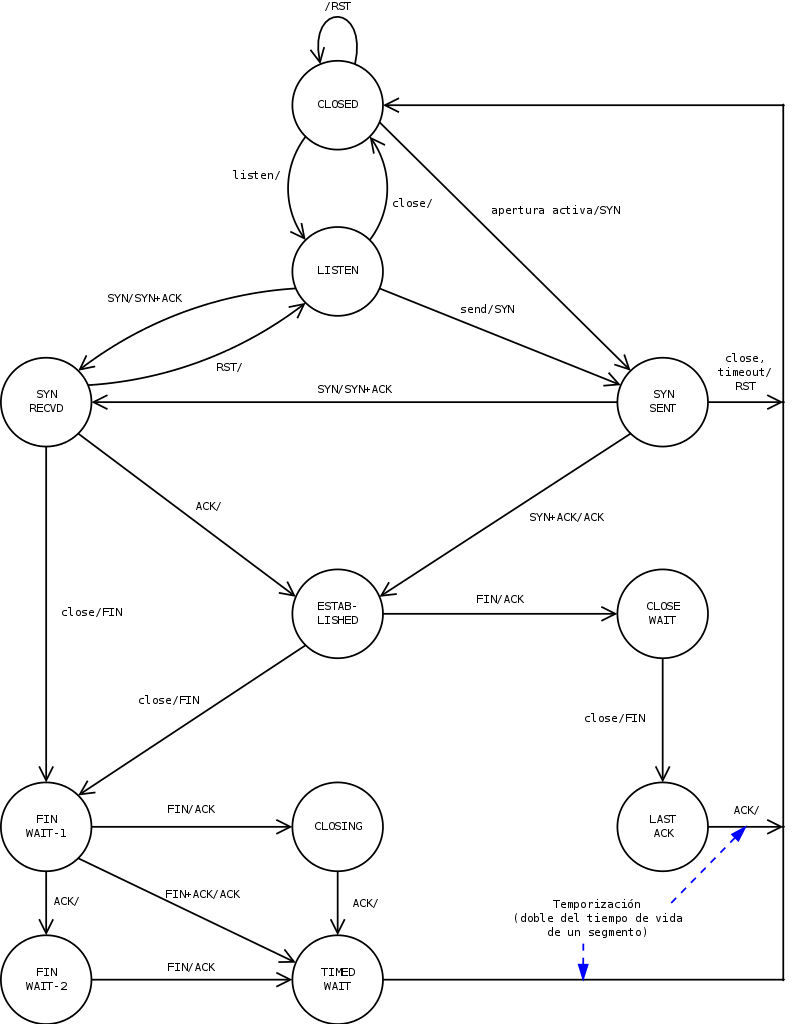
\includegraphics[width=0.98\textwidth]{img/EstadosTCP.png}
\end{figure}
\newpage
\subsection{Ventana deslizante}
TCP consigue transferencia fiable mediante el uso de la \textbf{ventana deslizante}.
\subsubsection{Parada y Espera vs. Ventana Deslizante}
En los protocolos de \textbf{parada y espera}, cuando el emisor envía un segmento, tiene que esperar a recibir un ACK antes de poder enviar el siguiente segmento.\\

Si después del timeout no llega el ACK, el emisor vuelve a enviar el segmento. Esto implica que un transmisor solo puede tener un elemento pendiente de reconocimiento, lo cual es bastante ineficiente.\\

Los protocolos de \textbf{ventana deslizante} por el contrario, pueden enviar varios segmentos sin esperar a recibir las confirmaciones de una en una.\\

La ventana deslizante permite:
\begin{itemize}
    \item La recepción de segmentos duplicados.
    \item La retransmisión de segmentos erróneos o perdidos.
    \item La recepción de segmentos fuera de orden.
\end{itemize}
\begin{figure}[H]
    \centering
    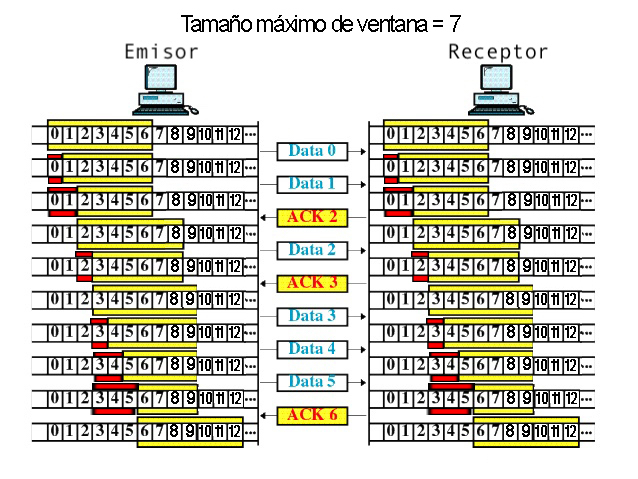
\includegraphics[width=\textwidth]{img/ventanasTCP.jpg}
    \caption{Intercambio de paquetes mediante ventana deslizante.}
\end{figure}
\subsubsection{Emisor}
\begin{itemize}
    \item Almacena los elementos pendientes de reconocimiento [marcados en rojo en el ejemplo]. El límite inferior de la ventana indica el primer segmento sin confirmar (si lo hay), o el siguiente segmento a enviar (si todos los segmentos están confirmados).
    \item Almacena también los elementos que pueden ser enviados [marcados en amarillo].
    \item El tamaño de la ventana siempre es igual al tamaño máximo [7 en el ejemplo]. Excepto cuando la aplicación no tiene tantos datos para enviar, en cuyo caso es menor.
\end{itemize}
\vspace{2cm}
\subsubsection{Receptor}
\begin{itemize}
    \item Almacena los elementos pendientes de ser consumidos por la aplicación [marcados en rojo en el ejemplo]. El límite inferior de la ventana indica el primer segmento sin ser consumido (si lo hay), o el siguiente segmento a recibir (si todos los segmentos están consumidos).
    \item Almacena también los elementos que pueden ser recibidos [marcados en amarillo].
    \item El tamaño de la ventana siempre es igual al tamaño máximo [7 en el ejemplo]. Excepto cuando la aplicación no tiene tantos datos para recibir, en cuyo caso es menor.
    \item Una vez los segmento son recibidos, el receptor envía un ACK, cuyo número indica el siguiente segmento a recibir.
    \item Para enviar los ACK se utiliza la técnica de \textbf{Piggybacking}, que consiste en incluir el ACK en otro segmento de datos que el receptor quiera enviar al emisor (ya que la comunicación es bidireccional).
\end{itemize}
\newpage
\subsection{Control de errores}
Vamos a ver cómo TCP resuelve algunas situaciones conflictivas.
\subsubsection{Recepción fuera de orden}
TCP controla la recepción de datos fuera de orden mediante confirmaciones (ACK) de la siguiente forma.
\begin{figure}[H]
    \centering
    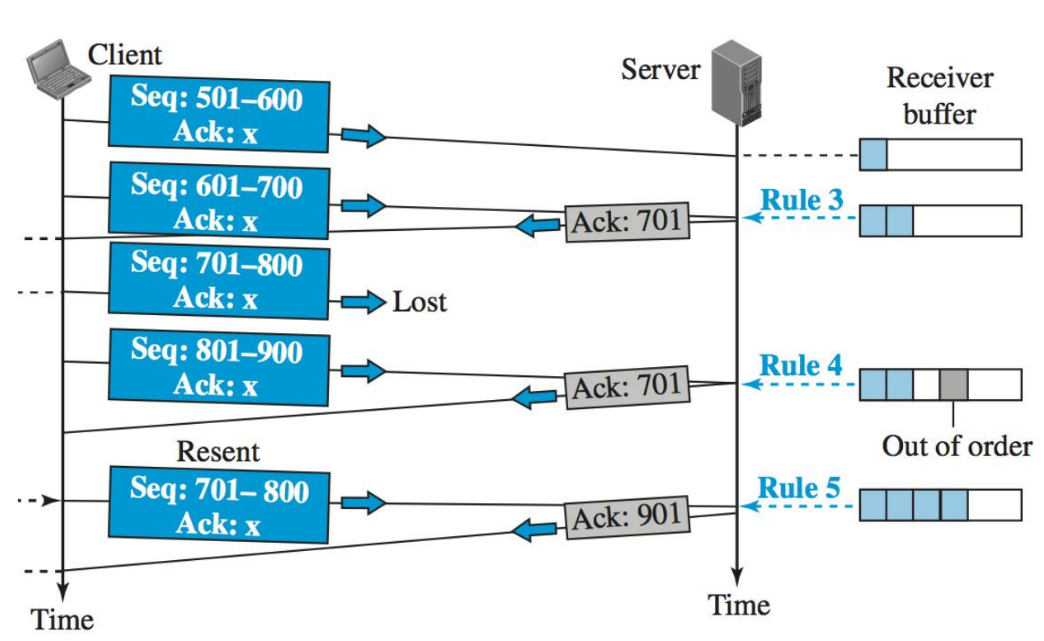
\includegraphics[width=\textwidth]{img/TCPooo.png}
    \caption{Recepción fuera de orden.}
\end{figure}
\begin{itemize}
    \item Si hay huecos, el receptor envía el ACK del primer hueco que tenga en el buffer.
    \item Si no hay huecos envía el ACK del siguiente segmento esperado.
    \item Los segmentos duplicados se confirman para prevenir pérdidas de ACK.
\end{itemize}
\subsubsection{Pérdida de un segmento}
¿Qué hacer cuando se pierde un segmento, o se recibe erróneamente? para ello TCP tiene dos \textbf{mecanismos de retransmisión}:
\begin{enumerate}
    \item \textbf{Temporizador de retransmisión:} si el emisor tiene segmentos sin confirmar, los reenvía al finalizar el temporizador. Si hay varios segmentos sin confirmar, el emisor reenvía el primero de la ventana.
        \begin{figure}[H]\centering
        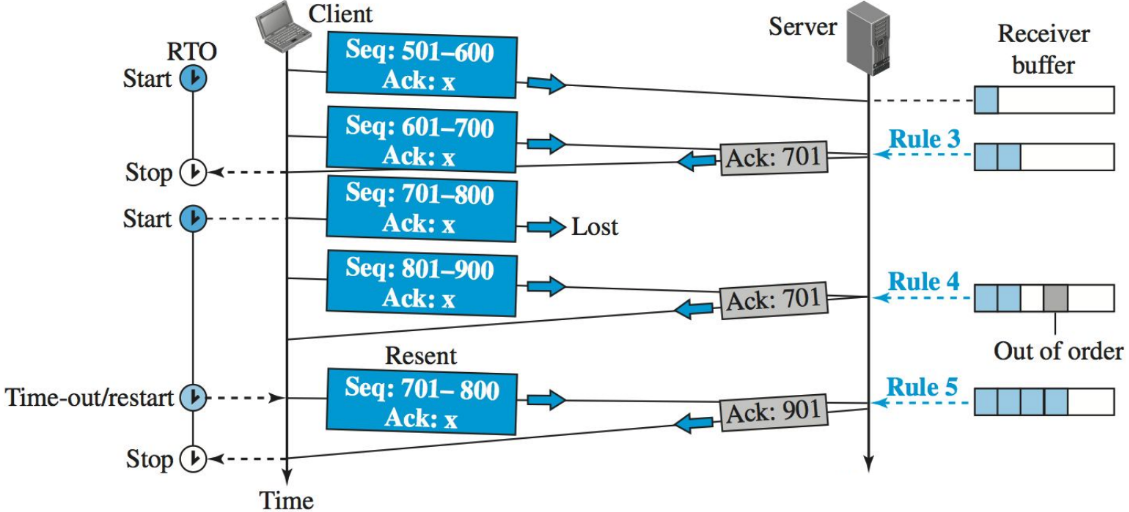
\includegraphics[width=\textwidth]{img/TCPTdRet.png}
        \caption{Temporizador de retransmisión.}\end{figure}
    \item \textbf{Retransmisión rápida:} si se reciben tres ACKs duplicados, el emisor reenvía el paquete.
        \begin{figure}[H] \centering
        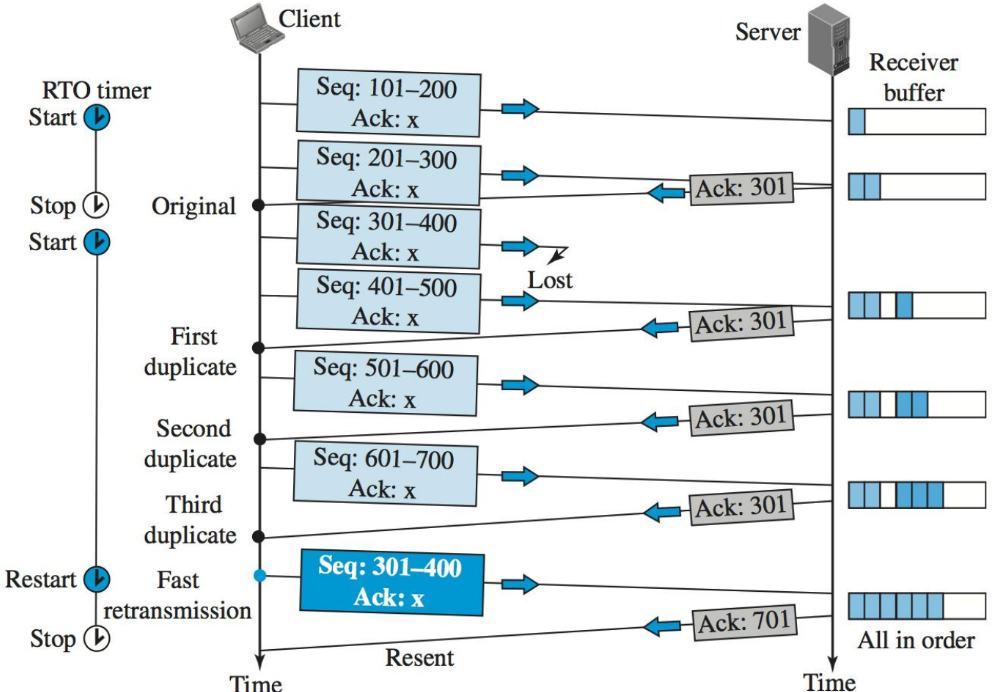
\includegraphics[width=\textwidth]{img/TCPRetRap.png}
        \caption{Retransmisión rápida.}\end{figure}
\end{enumerate}
\newpage
\subsubsection{Pérdida de un ACK}
Con respecto a la pérdida de ACKs se pueden dar dos situaciones.
\begin{itemize}
    \item \textbf{No expira el temporizador de retransmisión:} el emisor sigue enviando paquetes, por lo que si el siguiente ACK confirma un segmento posterior, también confirma todos los anteriores.
        \begin{figure}[H]\centering
        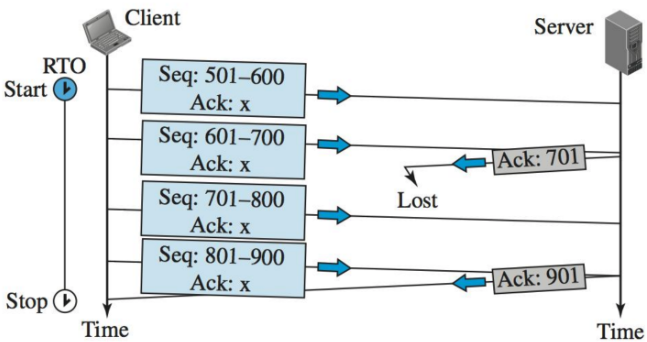
\includegraphics[width=\textwidth]{img/TCPACK1.png}
        \caption{No expira el temporizador de retransmisión.}\end{figure}
    \item \textbf{Expira el temporizador de retransmisión:} si el emisor no sigue enviando paquetes, cuando su temporizador de retransmisión expire, reenviará el paquete sin confirmar.
        \begin{figure}[H] \centering
        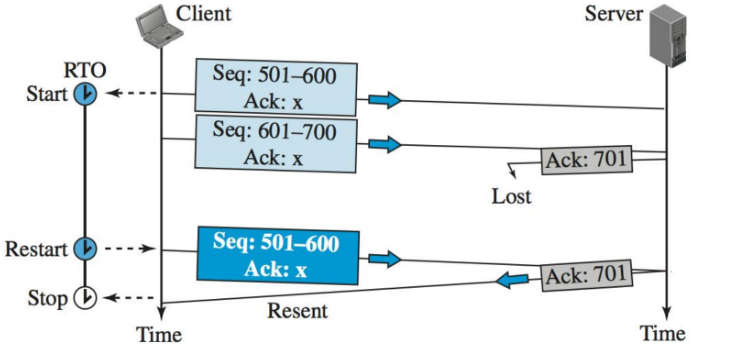
\includegraphics[width=\textwidth]{img/TCPACK2.png}
        \caption{Expira el temporizador de retransmisión.}\end{figure}
\end{itemize}
\begin{onepage}
\subsection{Temporizadores TCP}
TCP utiliza 4 temporizadores.
\begin{itemize}
    \item \textbf{Keepalive: }se utiliza para comprobar si un enlace está o no operativo. Cuando el temporizador expira (más de 2 horas, normalmente) envía una serie de señales \textit{keepalive}. Si no recive los ACK correspondientes, cierra la conexión.
    \item \textbf{TIMEWAIT: }en el cierre de conexión es el tiempo que espera la máquina que ha iniciado el cierre después de recibir el FIN (tanto en 3 como en 4 vías), para dar tiempo a la otra máquina a recibir el último ACK.
    \begin{figure}[H] \centering
    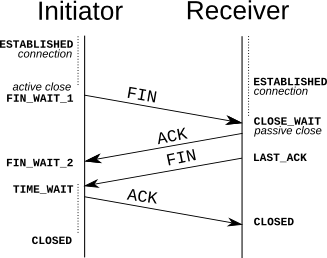
\includegraphics[width=0.5\textwidth]{img/TCP_TIMEWAIT.png}\end{figure}
    \item \textbf{Temporizador de persistencia: \label{tempers}}cuando el receptor advierte de un tamaño de ventana igual a 0, el emisor deja de enviar datos e inicia el temporizador de persistencia. El temporizador de persistencia se usa para proteger a TCP de una situación de interbloqueo que podría surgir si se pierde una actualización del tamaño de la ventana del receptor, y el emisor no puede enviar más datos hasta que reciba una nueva actualización del tamaño de la ventana del receptor. Cuando el temporizador expira, el emisor envía un pequeño paquete esperando un ACK, que le indique el nuevo tamaño de ventana.
    \item \textbf{Temporizador de retransmisión: }se utiliza cuando se espera un ACK del otro extremo. Veámoslo con más detalle.
\end{itemize}
\end{onepage}

\begin{onepage}
\begin{tcolorbox}[
title=Temporizador de retransmisión (TIMEOUT),
colback=cyan!5!white,
colframe=cyan!75!black,
fonttitle=\bfseries]
El tiempo de TIMEOUT se establece dinámicamente en función del tráfico de la red, y se pueden usar 3 algoritmos distintos para establecerlo.\\

El tiempo de ida y vuelta (\textbf{RTT}), es el tiempo transcurrido desde que se envía el
segmento hasta que se recibe el ACK. El RTT puede presentarse de tres formas distintas:
\begin{itemize}
    \item \textbf{RTT medido (RTTm): }es el RTT tal cual, por lo que puede experimentar grandes fluctuaciones. Por ejemplo si recibe un ACK acumulado, el RTTm se disparará.
    \item \textbf{RTT suavizado (RTTs): }es la media ponderada entre el RTTm y el último RTTS calculado. De forma que el primer RTTs = RTTm, y los siguientes valores dependen del RTTm actual y del RTTs anterior.
    \item \textbf{RTT desviación (RTTd): }Considera la variación del tiempo de ida y vuelta, y se calcula a partir del RTTm y del RTTs.
\end{itemize}

En éstos valores se basan los 3 \textbf{algoritmos} que puede usar el temporizador de retransmisión.
\begin{itemize}
    \item \textbf{Jacobson: }utiliza únicamente RTTs.
    \item \textbf{Jacobson/Karels: }mejora el anterior combinando RTTS y RTTD.
    \item \textbf{Karn: }se basa en el anterior se basa solo en ACKs de segmentos que fueron enviados solo una vez.
\end{itemize}
\end{tcolorbox}
\subsection{Control de flujo}
El control de flujo se utiliza para evitar desbordar el buffer del receptor cuando transmitimos muy rápido demasiados datos. Para ello TCP adaptará dinámicamente la ventana del emisor, dependiendo del tamaño de la ventana del receptor (anunciado cada ACK).\\

Si el receptor se queda sin espacio, su ventana tendrá tamaño = 0, y el emisor dejará de enviar datos. El emisor volverá a enviar datos de nuevo cuando el tamaño de la ventana del receptor vuelva a ser mayor que 0. Para saber el tamaño, utiliza el \underline{\hyperref[tempers]{temporizador de persistencia.}}

\end{onepage}
\subsubsection{Síndrome de la ventana tonta}
Ocurre cunado o bien el servidor genera datos a un ritmo muy lento, o bien el cliente consume los datos a un ritmo muy lento.\\
\begin{tcolorbox}[colback=white]
Para evitar la ventana tonta en el \textbf{emisor}, se inventó el \textbf{algoritmo de Nagle}:
\begin{itemize}
    \item Se envía el primer mensaje.
    \item Se espera a enviar los siguientes hasta que:
    \begin{enumerate}
        \item se recibe un ACK del receptor.
        \item se acumulan x bytes.
        \item expira el TIMEOUT.
    \end{enumerate}
\end{itemize}
\end{tcolorbox}
\begin{tcolorbox}[colback=white]
Para evitar la ventana tonta en el \textbf{receptor}, se inventó el \textbf{algoritmo de Clark}:
\begin{itemize}
    \item Se anuncia tamaño de ventana 0 hasta que:
    \begin{enumerate}
        \item Se puede recibir un segmento completo.
        \item Se ha liberado la mitad del buffer de recepción.
    \end{enumerate}
\end{itemize}
\end{tcolorbox}


\subsection{Control de la congestión}
Cuando se pierde paquetes en Internet, la mayoría de las veces se debe a un problema de congestión en algún punto de la red: puede ocurrir que el router no pueda procesar paquetes al ritmo al que los recibe. Entonces, empieza a descartar paquetes.\\

El control de la congestión y el flujo son dos mecanismos diferentes. El control de flujo se encarga de ajustar la transmisión en el receptor, mientras que el \textbf{control de congestión} puede aparecer en cualquier punto de la red. Si un router no es capaz de gestionar todos los paquetes, empieza a descartar.\\

El emisor utiliza el ritmo de llegada de confirmaciones para regular el ritmo de
envío de segmentos de datos. Para ello utiliza la Ventana de congestión \textbf{(CW)}.\\

La ventana de congestión es complementaria a la ventana de recepción \textbf{(RW)} usada para el control de flujo.
\begin{itemize}
    \item En una situación de no congestión (sin pérdida o retraso de segmentos) la ventana de congestión alcanza el mismo tamaño que la ventana de recepción \textbf{(CW = RW)}.
    \item Cuando se produce una situación de congestión el tamaño de \textbf{CW} se va reduciendo progresivamente.
    \item Cuando la situación de congestión desaparece, el tamaño de CW se va aumentando progresivamente
    \item El número máximo de bytes que puede enviar el emisor \textbf{(AW, Allowed Window)} es el mínimo de ambos tamaños de ventana:\\
    \begin{center}
        $AW = min ( RW, CW )$
    \end{center}
\end{itemize}

\subsubsection{Fases del control de la congestión}
La transmisión comienza con CW = 1.
\begin{enumerate}
    \item \textbf{Fase de arranque lento:} el tamaño aumenta exponencialmente con cada segmento enviado hasta llegar a un umbral (SST, Slow Start Threshold). Inicialmente, el valor del SST suele ser de 64 Kbytes.
    \item \textbf{Fase de evitación de congestión:} Cuando se confirman todos los segmentos de la ventana la CW aumenta en +1 (crecimiento lineal).
    \item \textbf{Fase constante:} si la CW alcanza el mismo tamaño que la ventana de flujo (RW), el tamaño se mantiene.
\end{enumerate}
    \begin{figure}[H] \centering
    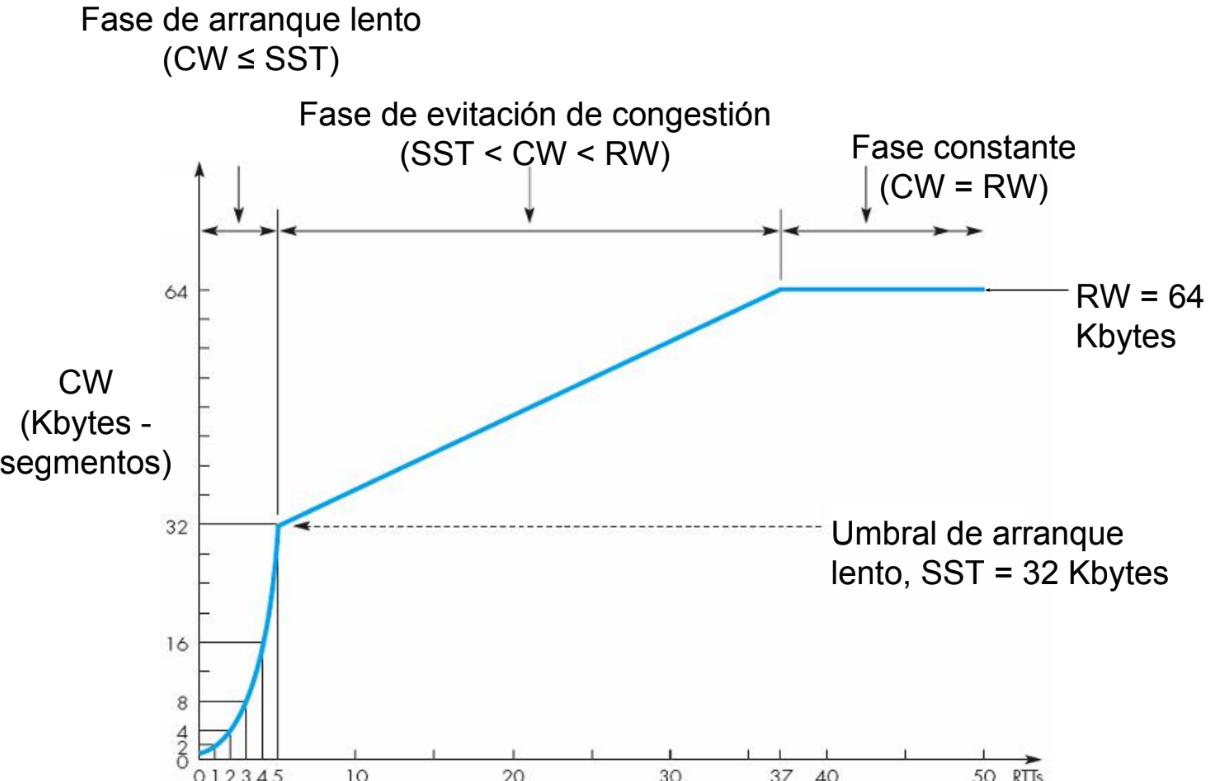
\includegraphics[width=0.8\textwidth]{img/TCP_FasesCong.png}\end{figure}
    
\subsubsection{Mecanismos de control de la congestión}
Durante la conexión pueden aparecer congestiones que se detectan de forma indirecta de dos formas distintas:
\begin{itemize}
    \item Se reciben \textbf{3 ACKs duplicados}. Esto indica un nivel de congestión leve, ya que sigue habiendo tráfico en la red.\\
    
    Ante esta situación se activa el método de recuperación rápida (fast recovery):
    \begin{enumerate}
        \item Se divide el valor de CW a la mitad.
        \item Se ejecuta el método de evitación de colisiones a partir de ese valor de CW.
    \end{enumerate}
        \begin{figure}[H] \centering
        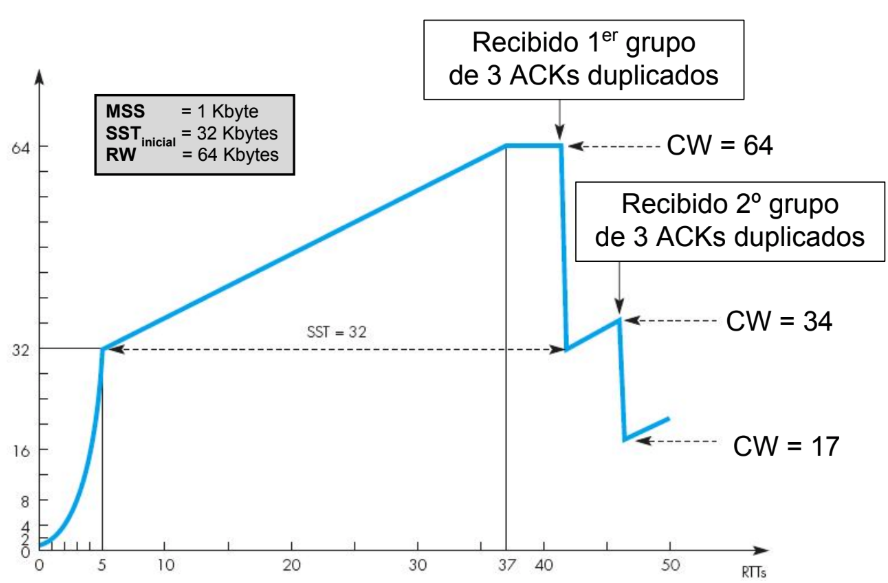
\includegraphics[width=0.8\textwidth]{img/TCP_3acks.png}\end{figure}
    \item \textbf{Expira el temporizador} de retransmisión. Esto indica un nivel de congestión elevado, ya que se interpreta que el tráfico en la red está interrumpido.
    En este caso se realizan las siguientes acciones:
    \begin{enumerate}
        \item Se inicializa el tamaño de la ventana de congestión a CW = 1.
        \item Se reduce el umbral de arranque lento (SST), fijándolo a la mitad del valor que tenía la CW antes de producirse el timeout.
        \item Se ejecuta el método de arranque lento a partir de CW = 1.
    \end{enumerate}
        \begin{figure}[H] \centering
        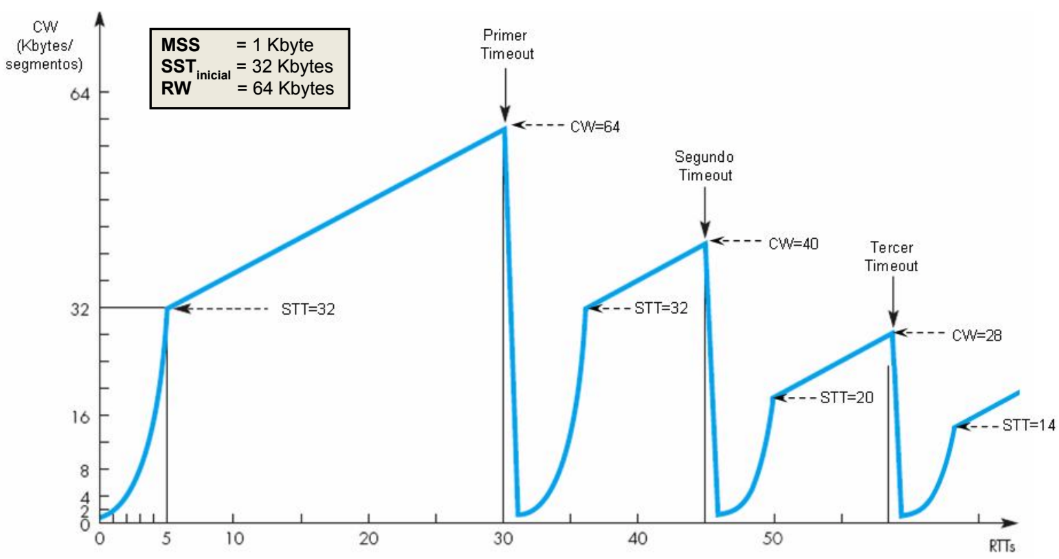
\includegraphics[width=0.9\textwidth]{img/TCP_congtimeout.png}\end{figure}
\end{itemize}
%%%%%%%%%%%%%%%%%%%%%%%%%%%%%%%%%%%%%%%%%%%%%%%%%%%%%%%%%%%%%%%%
\begin{onepage}


\section{Servicios de Red: Filtrado de paquetes.}
\subsection{Firewall y filtrado de paquetes.}
Un \textbf{Firewall:} es un dispositivo configurado para permitir, limitar, cifrar o descifrar el tráfico de red en base a un conjunto de normas.

\subsubsection{Tipos de Firewall.}
\begin{itemize}
    \item \textbf{En función del estado (stateless/stateful): }Si el filtrado se basa únicamente en la cabecera del paquete o además considera el estado de la conexión.
    \item \textbf{En función de la capa (de red o de aplicación):} consideran informacion no solo de las cabeceras si no de los datos(que normalmente pertenecen a protocolos de aplicación como http). Este tipo de firewalls se dice que realizan DPI (Deep packet inspection).
\end{itemize}

\subsection{Iptables.}
\textbf{Netfilter} es una herramienta del kernel de Linux que proporciona filtrado y modificación de paquetes.\\

El componente más popular construido sobre Netfilter es \textbf{iptables}, una herramienta de cortafuegos que permite no solamente filtrar paquetes, sino también realizar traducción de direcciones de red (NAT).\\
\begin{tcolorbox}[
colback=yellow!5!white,
colframe=yellow!75!cyan,
fonttitle=\bfseries]
Para tener clara la estructura de iptables, primero debemos entender los siguientes conceptos:
\begin{itemize}
    \item \textbf{Regla: }define qué hacer con un paquete que cumple unas determinadas características. \textit{Por ejemplo descartar los paquetes con una IP destino determinada.}
    \item \textbf{Cadena: }es una lista ordenada de reglas que se aplican sobre los paquetes en distintos puntos del proceso del paquete.
    \item \textbf{Tabla: }es un conjunto de cadenas, cada una destinada a diferentes tipos de procesamiento sobre cada paquete.
\end{itemize}
\end{tcolorbox}
\end{onepage}

\begin{onepage}
\subsubsection{Tablas predefinidas.}
\begin{itemize}
    \item \textbf{Tabla filter: }es la tabla por defecto. Contiene tres cadenas, que clasifican los paquetes:
        \begin{itemize}
            \item INPUT: paquetes recibidos.
            \item OUTPUT: paquetes generados.
            \item FORWARD: paquetes que atraviesan el sistema.
        \end{itemize}
    
    \item \textbf{Tabla NAT: }reescribe direcciones origen/destino y los puertos de un paquete. Contiene tres cadenas.
            \begin{itemize}
                \item PREOUTING: se aplica a paquetes de entrada antes de pasar por la tabla de encaminamiento local.
                \item POSTROUTING: se aplica a paquetes justo antes de ser enviados, modifica la direccion de origen de los paquetes.
                \item OUTPUT: similar a la cadena homonima de la tabla filter.
            \end{itemize}
    \item \textbf{Tabla Mangle: }sirve para cambiar algunos campos del paquete. Contiene las cinco cadenas anteriormente descritas.
    \end{itemize}
    \begin{figure}[H]
        \centering
        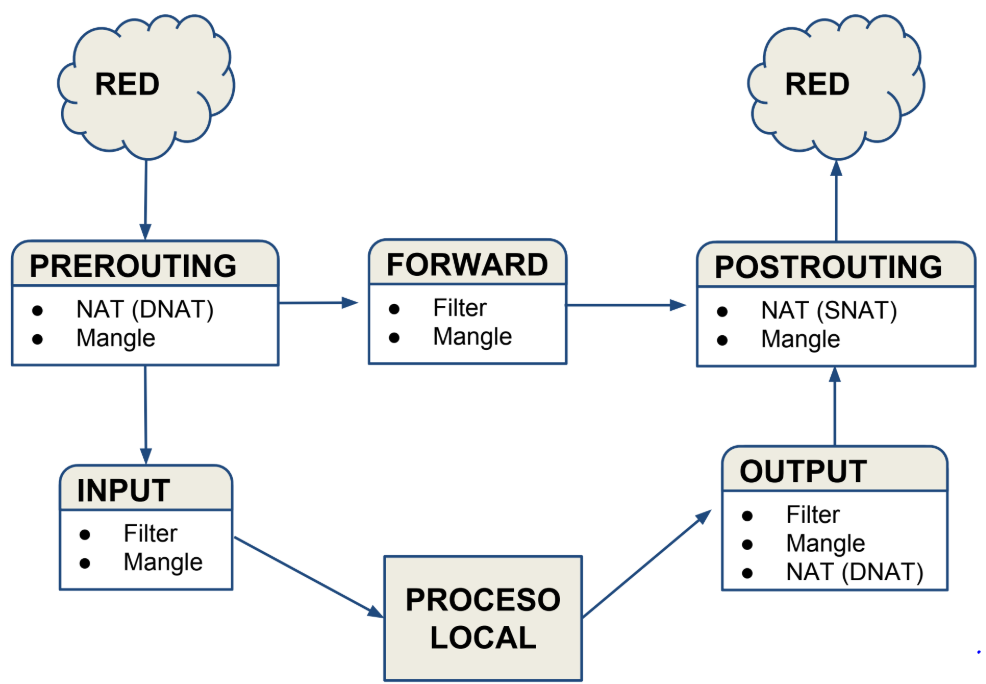
\includegraphics[width=0.8\textwidth]{img/GraficoCadenas.PNG}
        \caption{Diagrama de cadenas}
    \end{figure}
    \end{onepage}
\subsubsection{Definición de Reglas.}
    Las reglas se pueden definir según la información del paquete o según el estado de la conexión. Debe incluir la \textbf{cadena} a la que se añade la regla y un \textbf{objetivo} (qué hacer si el paquete coincide).
    
    \begin{table}[H]\centering\begin{tabular}{|l|l|}\hline
    \multicolumn{2}{|c|}{\cellcolor[HTML]{000000}{\color[HTML]{FFFFFF} \textbf{Política por defecto}}} \\ \hline
    -P INPUT & \multirow{3}{*}{Política por defecto} \\ \cline{1-1}
    -P OUTPUT &  \\ \cline{1-1}
    -P FORWARD &  \\ \hline
    \end{tabular}\end{table}
    
    \begin{table}[H]\centering\begin{tabular}{|l|l|}\hline
    \multicolumn{2}{|c|}{\cellcolor[HTML]{000000}{\color[HTML]{FFFFFF} \textbf{Cadena}}} \\ \hline
    -A INPUT & Añade regla a cadena de entrada \\ \hline
    -A OUTPUT & Añade regla a cadena de salida \\ \hline
    -A FORWARD & Añade regla a la cadena forward (sólo en caso de routers) \\ \hline
    \end{tabular}\end{table}

    \begin{table}[H]\centering\begin{tabular}{|l|l|}\hline
    \multicolumn{2}{|c|}{\cellcolor[HTML]{000000}{\color[HTML]{FFFFFF} \textbf{Objetivo}}} \\ \hline
    -j DROP &  \\ \hline
    -j ACCEPT &  \\ \hline
    -j REJECT & igual que DROP pero envía un ICMP de un tipo que puede definirse \\ \hline
    -j LOG &  \\ \hline
    \end{tabular}\end{table}  
    
    \begin{table}[H]\centering\begin{tabular}{|c|}\hline
    \rowcolor[HTML]{000000}  {\color[HTML]{FFFFFF} \textbf{Opciones}} \\ \hline
    Consultar el manual de iptables \\ \hline
    \end{tabular}\end{table}
    
    \begin{figure}[H]
        \centering
        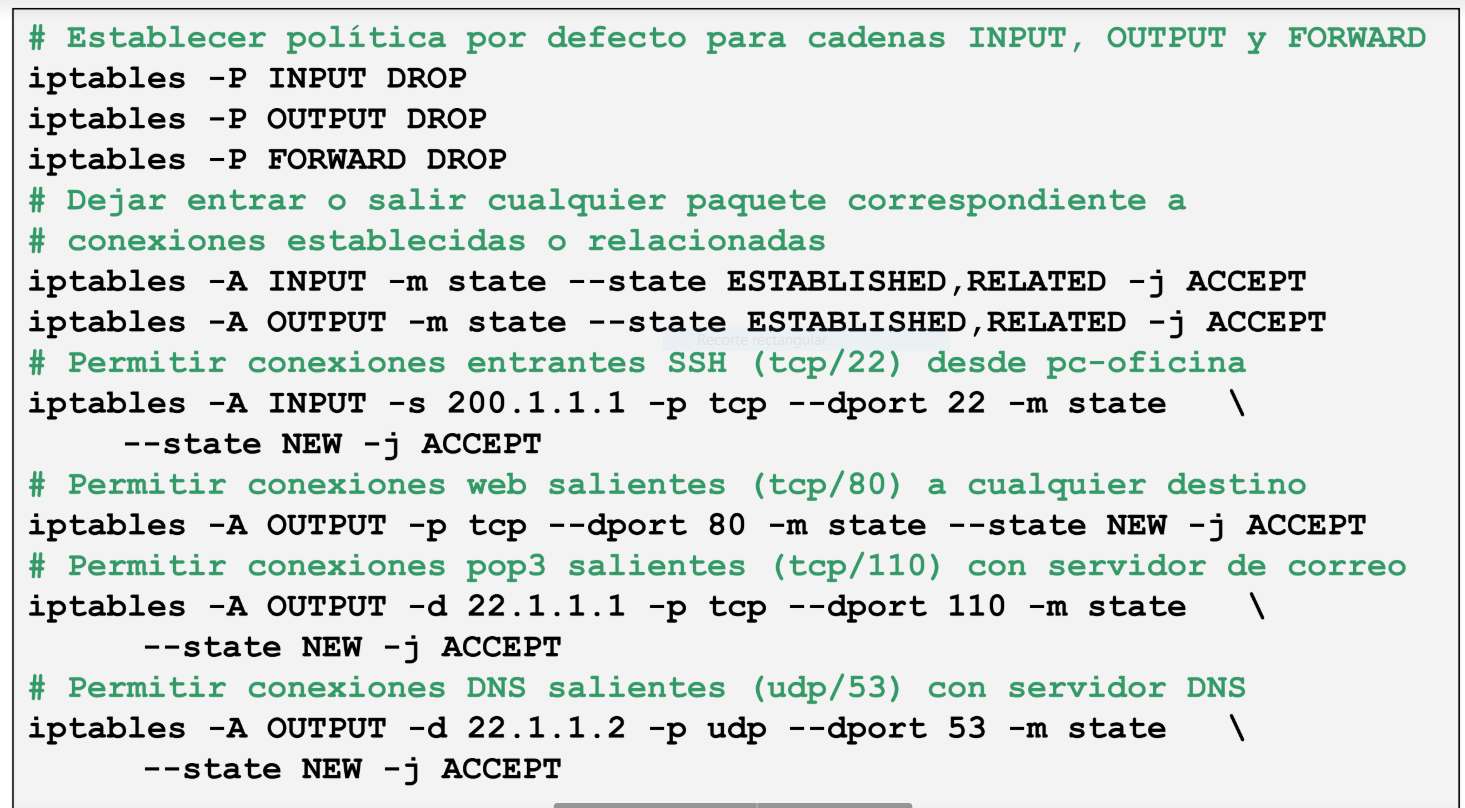
\includegraphics[width=\textwidth]{img/EjemplosReglas.PNG}
        \caption{Ejemplos de reglas}
    \end{figure}
    
\begin{onepage}
    \subsubsection{NAT}
    \textbf{NAT: Network Address Translation:} permite dar acceso a Internet a máquinas en redes privadas realizando traducciones.\\
    
    NAT almacena una \textbf{tabla} que relaciona las direcciones privadas con las direcciones públicas.\\
    
    Existen los siguientes modos de funcionamiento:
    \begin{itemize}
        \item \textbf{Estáticas: }consiste en una asignación fija de N direcciones privadas a N direcciones públicas.
        \item \textbf{Dinámicas: }consiste en una asignación de N direcciones privadas a M direcciones públicas, donde $(M < N)$. Por tanto las N direcciones privadas se disputan las M direcciones públicas.
        \item \textbf{Sobrecarga o NAPT: }asigna N direcciones privadas a 1 dirección pública.
        \begin{figure}[H]\centering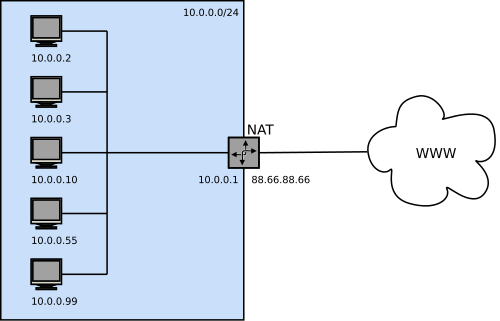
\includegraphics[width=0.7\textwidth]{img/NAT.png}\end{figure}
        \begin{itemize}
            \item Para paquetes de salida se utiliza la técnica de \textbf{Masquerading}: traduce la dirección privada a la dirección pública asignada al router. 
            \item Para los paquetes entrantes se utiliza la técnica de \textbf{Port forwarding, o servidores virtuales}, el router tiene una tabla con unas traducciones que depende del \textbf{número de puerto} asignado con el router.
        \end{itemize}
    \end{itemize}
\end{onepage}
%%%%%%%%%%%%%%%%%%%%%%%%%%%%%%%%%%%%%%%%%%%%%%%%%%%
\section{DNS}
\begin{figure}[H]\centering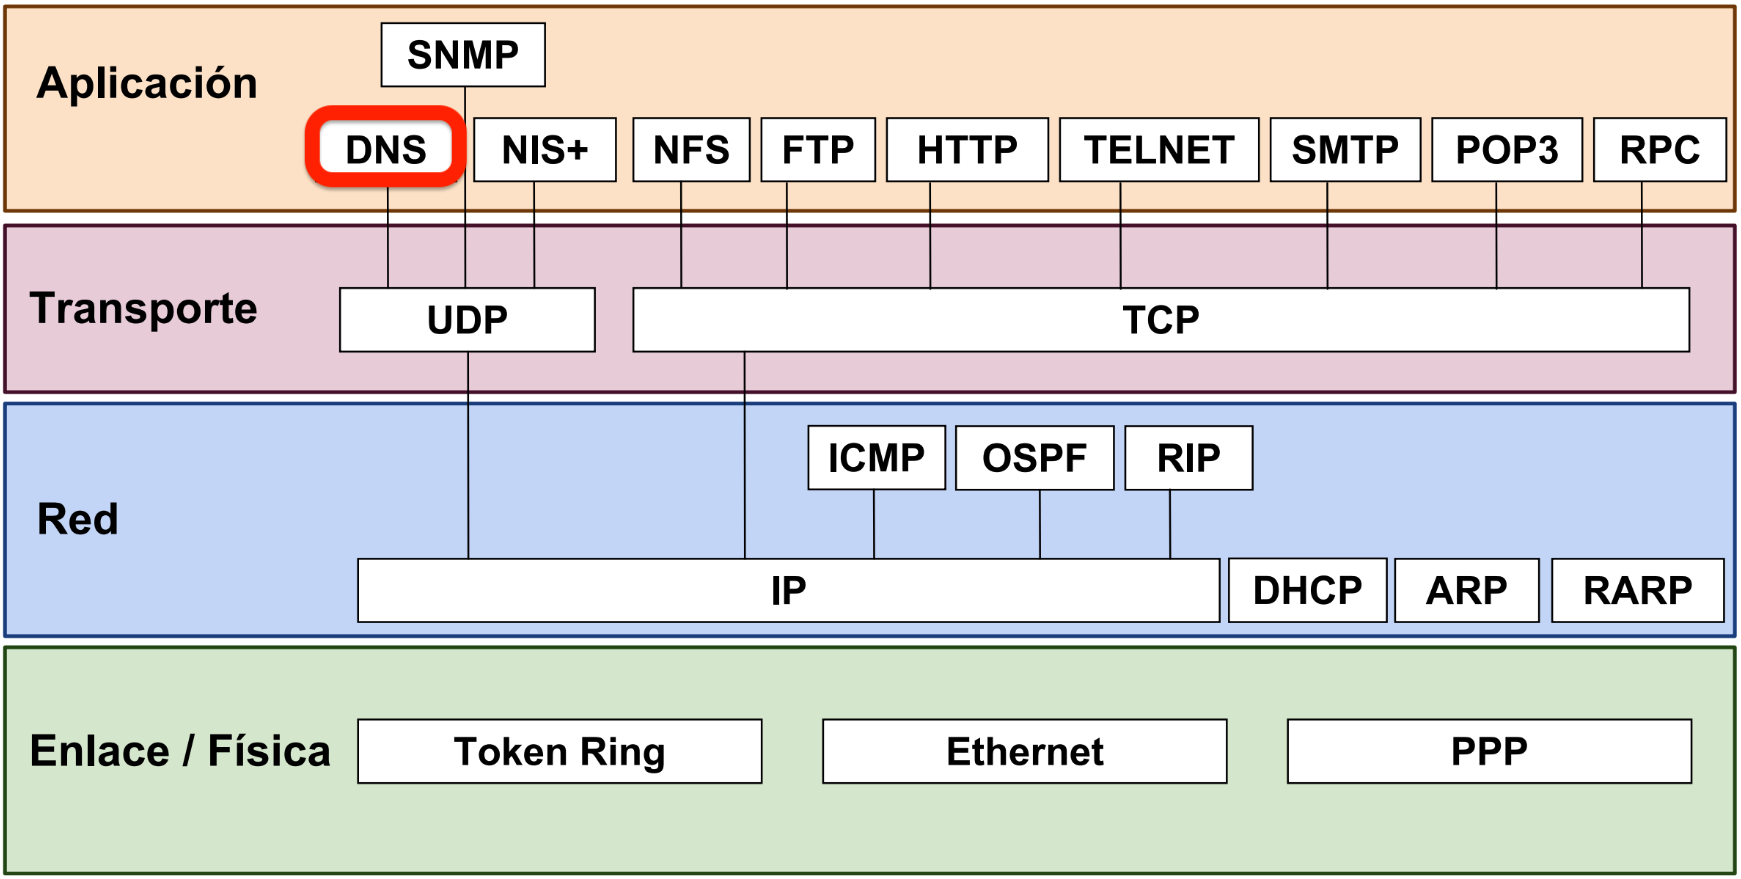
\includegraphics[width=0.7\textwidth]{img/DNS.png}
\end{figure}
\textbf{DNS (Domain Name System)}, es un sistema de nomenclatura  para dispositivos conectados a redes IP. Su función más importante es \enquote{traducir} nombres inteligibles para las personas en identificadores binarios asociados con los equipos, con el propósito de poder localizar y direccionar estos equipos mundialmente.\\

El servidor DNS utiliza una \textbf{base de datos distribuida} que almacena información asociada a nombres de dominio. DNS también define un protocolo de red.

\subsection{Zonas y dominios.}
Un nombre de dominio usualmente consiste en dos o más etiquetas, separadas por puntos. \textit{Por ejemplo, www.ucm.es.}

\[(root) \rightarrow (es) \rightarrow (ucm)\]\\
\textit{\enquote{es}} es un subdominio de primer nivel, que pueden ser generales (com, gov, net..) o de país (fr, es, uk...).\\

\textit{\enquote{ucm}} es un subdominio de segundo orden, etc...\\

Una \textbf{zona} DNS es una parte del espacio de nombres que se delega a una entidad legal. Cuando un navegador web necesita encontrar la dirección IP para un nombre de host, realiza una búsqueda de DNS en el servidor DNS que administra la zona para ese nombre de host.\\

Un \textbf{FQDN} (fully qualified domain name) es un nombre que incluye el nombre de la computadora y el nombre de dominio asociado a ese equipo. Por ejemplo, dada la computadora llamada \enquote{serv1} y el nombre de dominio \enquote{bar.com.}, el FQDN será \enquote{serv1.bar.com.}
\newpage
\subsection{Datagrama DNS}
\begin{figure}[H]\centering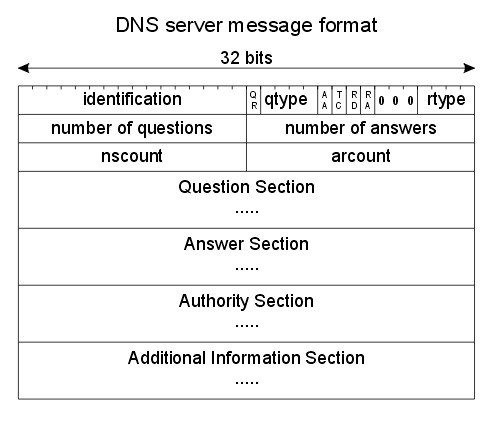
\includegraphics[width=0.7\textwidth]{img/DNS_Datagram.jpg}
\end{figure}
\begin{itemize}
    \item La \textbf{Cabecera} se divide en 6 campos, que permiten identificar el datagrama y determinar su contenido.
    \item Las secciones \textbf{Pregunta y Respuesta} incluye el nombre de dominio y el tipo de registro por el que se pregunta.
    \item Sección de \textbf{Autoridad} especifica los servidores de nombre oficiales de la zona por la que estamos preguntando.
    \item La sección \textbf{Adicional} incluye registros que pueden ser de ayuda (resolver)
\end{itemize}
\subsection{Características del protocolo DNS}
\begin{enumerate}
    \item La base de datos DNS se estructura en \textbf{registros}, que son la información básica que se intercambia y cachea en los servidores. DNS gestiona diferentes tipos de registros para almacenar servidores de nombres, asignaciones nombre-IP, etc...
    \item \textbf{BIND} es la implementación DNS más usada y es Open Source.
    \item Los datagramas DNS se encapsulan en \textbf{datagramas UDP}, aunque se puede utilizar TCP en algunos casos (como obtener toda la información de un servidor, o si la respuesta tiene más de 512 bytes)\\
    
    \item Ante una consulta DNS, se busca en primer lugar si dispone de la respuesta en la memoria caché. En caso contrario, se inicia la búsqueda de manera recursiva. Una vez encontrada la respuesta, el servidor DNS guardará el resultado en su memoria caché para futuros usos y devuelve el resultado.
    \begin{figure}[H]\centering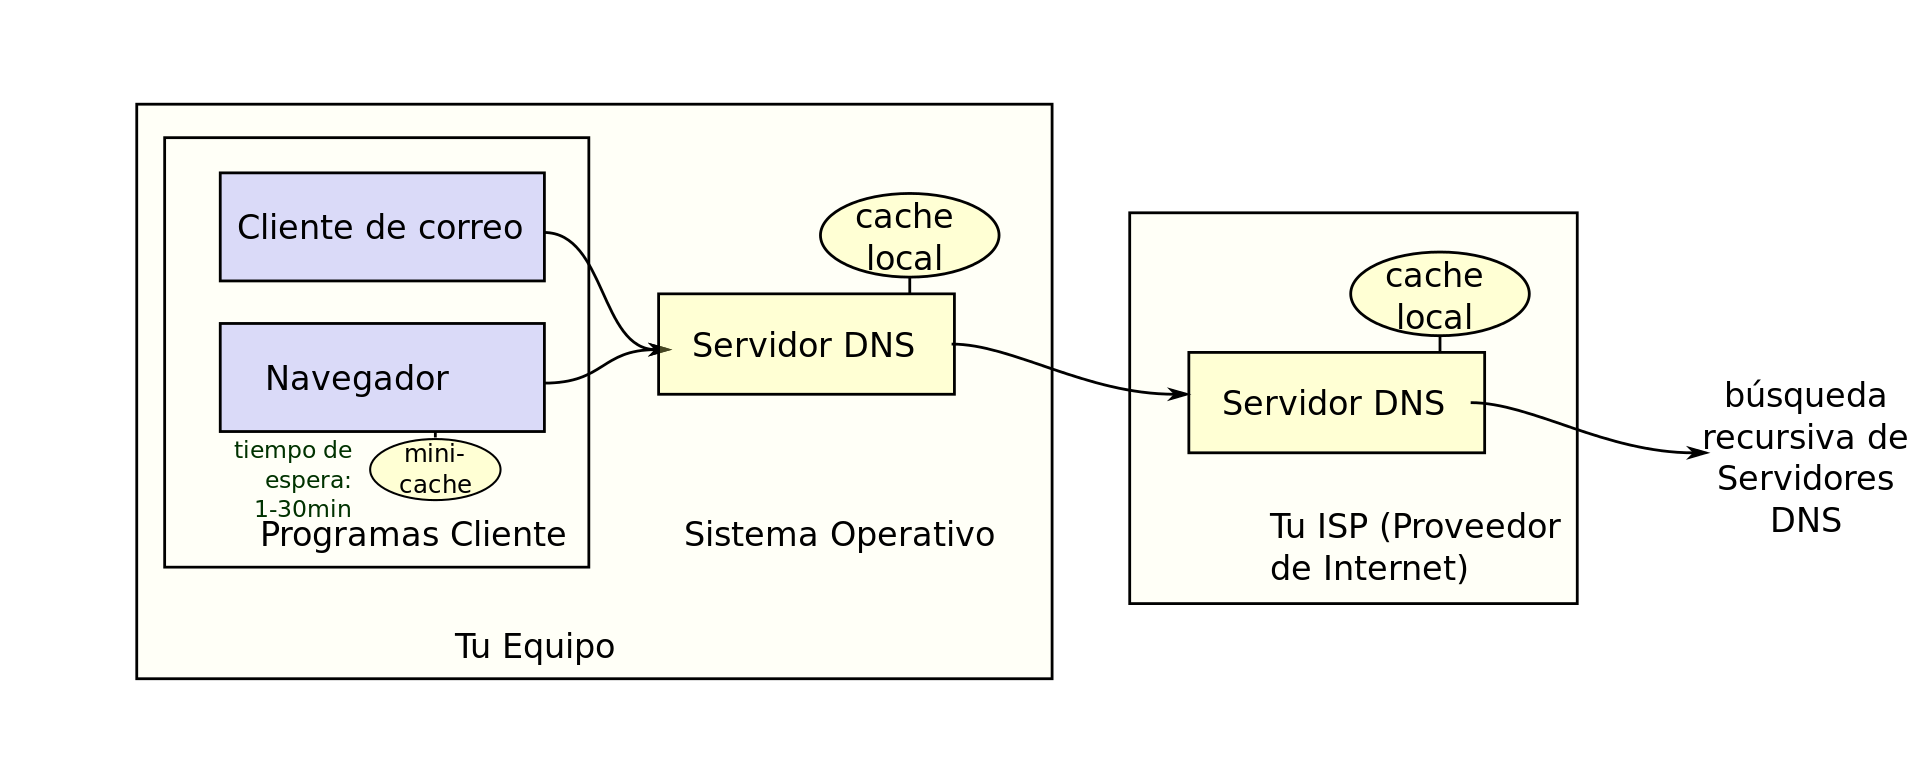
\includegraphics[width=\textwidth]{img/DNS_Busqueda.png}\end{figure}
    \item \textbf{Cachear} la resolución de direcciones mejora notablemente la eficiencia. La relación nombre-IP es prácticamente estática, por lo que las respuestas se cachean durante TTL (“time-to-live”) que varía según el nivel al que se encuentren, por ejemplo:
    \begin{itemize}
        \item Servidores de la zona \enquote{.es}, 2 días.
        \item Servidores del dominio \enquote{rediris.es}, 1 día.
        \item IP de \enquote{www.rediris.es}, 2 horas.
    \end{itemize}
    \item Existen los siguientes \textbf{Tipos de servidores:}
    \begin{itemize}
        \item \textbf{Autoritativos: }Representan oficialmente a la zona.
        \begin{itemize}
            \item Primarios o maestros: tienen la copia oficial en disco de la BD.
            \item Secundarios o esclavos: obtienen la BD de los primarios (zone transfer).
        \end{itemize}
        \item \textbf{De cache: }Guardan los resultados de las búsquedas realizadas. No tienen ningún registro DNS propio, ni son autoritativos para ninguna zona.
        \item \textbf{No recursivos: }cuando no disponen el registro de la consulta devuelven una referencia al servidor de nombres que puede tenerlo. Los servidores autoritativos suelen ser no recursivos.
        \item \textbf{Recursivos: }resuelven cada referencia hasta devolver la respuesta al cliente. En la configuración de los clientes deben usarse servidores recursivos.
    \end{itemize}
    \item La \textbf{base de datos DNS} consiste en archivos de texto  mantenidos en el servidor primario de la zona. La base de datos se compone de los siguientes registros:
    \begin{itemize}
        \item \textbf{SOA: }marca el comienzo de definición de una zona.
        \item \textbf{NS: }especifica los servidores autoritativos para la zona e incluye los servidores de nombres de los subdominios delegados a otras organizaciones.
        \item \textbf{A: }El registro Address (A para IPv4 y AAAA para IPv6) es la base de DNS. Incluye la traducción directa (nombre $\rightarrow$ IP)
        \item \textbf{PTR: }El registros Pointer contiene la traducción inversa (IP $\rightarrow$ nombre)
        \item \textbf{MX: }es usado por los sistemas de correo para encaminar los mensajes eficientemente. Permite recibir de forma centralizada el correo de una organización.
        \item \textbf{CNAME: } permite definir un alias para el nombre canónico. Deben siempre apuntar a un dominio (nunca a una IP).
    \end{itemize}
    \item El comando \textbf{dig} se puede usar para realizar consultas DNS.
\end{enumerate}
%%%%%%%%%%%
\begin{onepage}
\section{Protocolo IPv6}
\begin{figure}[H]
    \centering 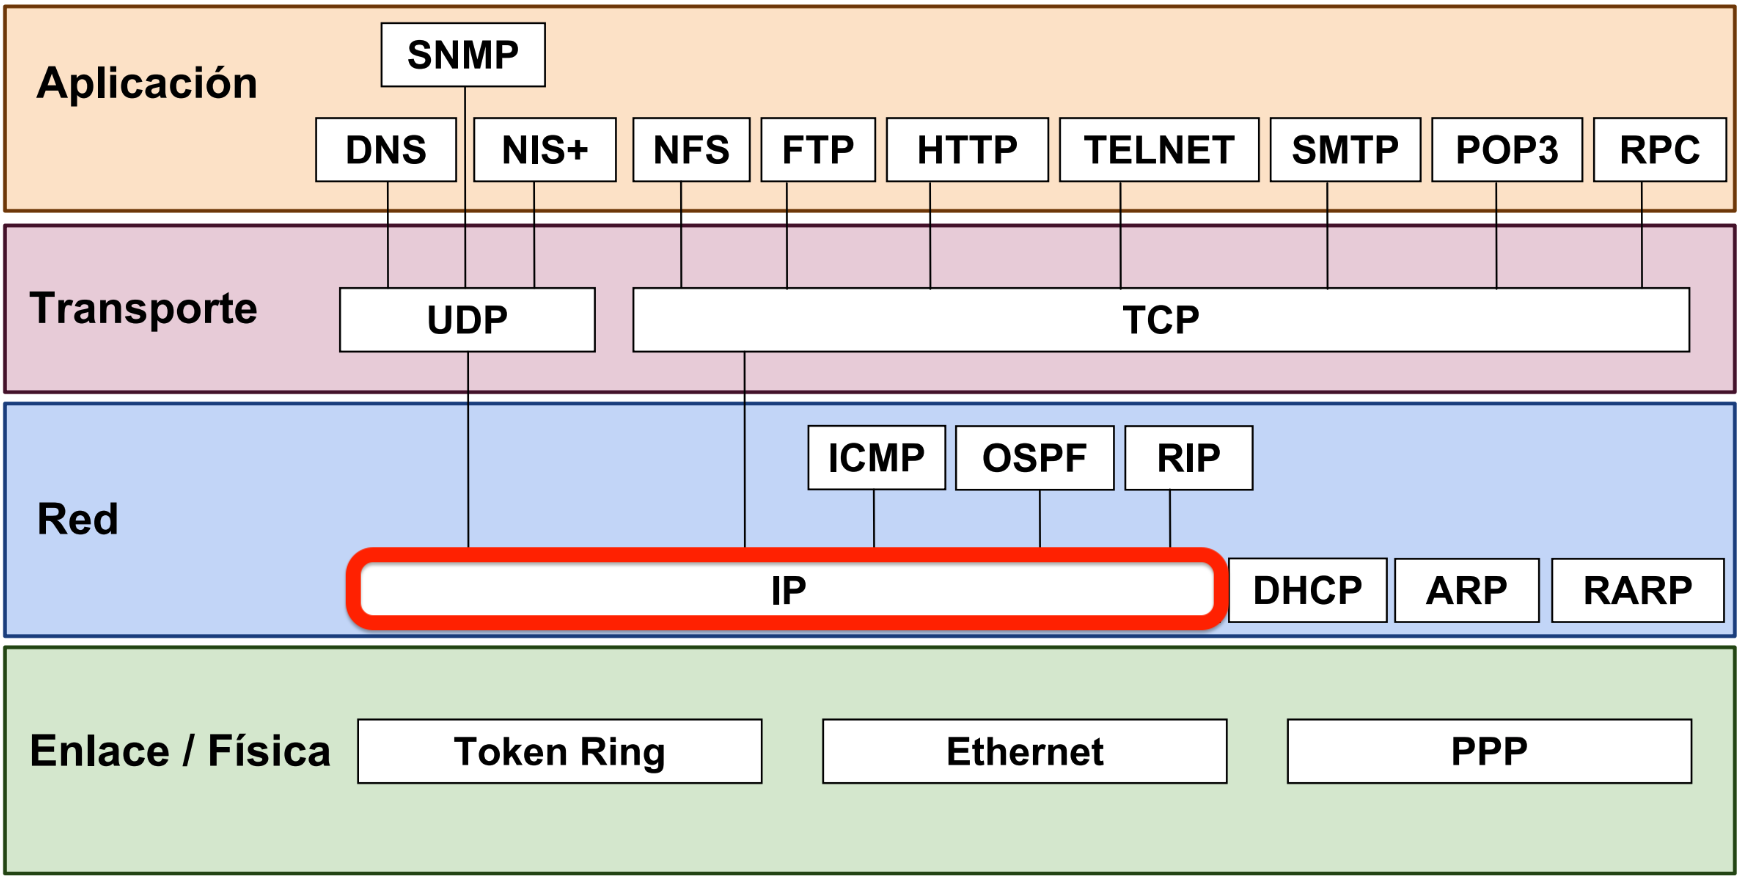
\includegraphics[width=0.7\textwidth]{img/IP.png}
\end{figure}
IPv6 es una versión del protocolo IP, creada como respuesta a las limitaciones de IPv4. Algunas de éstas limitaciones son:
\begin{itemize}
    \item El agotamiento de direcciones.
    \item El formato complejo de la cabecera.
    \item Problemas de seguridad.
\end{itemize}
A pesar de que IPv6 es usable desde hace años, a día de hoy IPv4 es el protocolo dominante en internet. Por ello, éstas limitaciones se han ido solucionando con parches durante los últimos años. \textit{Por ejemplo se ha adaptado la seguridad de IPv6 a IPv4.}
\subsection{IPv4 vs IPv6}
Frente a IPv4, IPv6 presenta algunas ventajas:
\begin{itemize}
    \item El espacio de direcciones es mucho mayor (128 bits, comparado con los 32 bits de IPv4).
    \item El formato de cabecera se simplifica, con lo que los routers son capaces de procesar más rápido.
    \item No se necesita DHCP, IPv6 es capaz de hacer su trabajo.
    \item IPv6 elimina las direcciones broadcast y las implementa como un caso especial de multicast.
    \item Proporciona opciones de seguridad tanto para autenticación como para cifrado.
    \item Implementa las direcciones Anycast, que envía el datagrama a la máquina más cercana.
    \item Da soporte para tráfico en tiempo real. \textit{Por ejemplo: VoIP.}
\end{itemize}
\end{onepage}
\begin{onepage}
\subsection{Direcciones IPv6}

\begin{table}[H]\centering\begin{tabular}{|c|c|}\hline\rowcolor[HTML]{FFCC67}
IPv4 & IPv6 \\ \hline
Unicast & Unicast \\ \hline
Multicast & Multicast \\ \hline
Broadcast & Anycast \\ \hline
\end{tabular}\end{table}
Un paquete dirigido a una dirección \textbf{unicast} se entregará únicamente al interfaz identificado con dicha dirección IP.\\

Las direcciones \textbf{multicast} identifican a un grupo de interfaces. Un paquete dirigido a una dirección multicast se entrega a todos los interfaces
identificados con esa dirección.\\

IPv6 no implementa broadcast, el mismo efecto puede lograrse enviando un paquete al grupo de multicast de enlace-local todos los nodos (all hosts). Por lo tanto, no existe el concepto de una dirección de broadcast y así la dirección más alta de la red (la dirección de broadcast en una red IPv4) es considerada una dirección normal en IPv6.\\

Las direcciones \textbf{anycast} son asignadas del espacio de direcciones unicast. De esta forma, las direcciones anycast no se pueden distinguir sintácticamente de las unicast. Cuando una dirección unicast es asignada a más de una interfaz, esta se convierte en una dirección anycast.

\subsubsection{Notación de direcciones.}
IPv6 usa la notación \textbf{hexadecimal}.
\begin{itemize}
    \item La dirección se divide en 8 grupos de 16 bits.
    \item Cada grupo se escribe en hexadecimal con 4 dígitos.
    \item Los grupos se separan por \enquote{:}.
    \item La longitud del prefijo se denota en CIDR.
    \item Existen algunos prefijos reservados, por ejemplo para direcciones multicast o ULA.
    \item Los 64 bits menos significativos determinan el ID del interfaz (distinto del host), que permite relacionar la dirección IP de red con la dirección MAC.
    \end{itemize}
    Como se generan direcciones muy largas, se usan algunos métodos para abreviar.
    \begin{itemize}
    \item Omitir los ceros a la izquierda de cada grupo.
    \item Las cadenas de ceros seguidos se pueden comprimir con el símbolo \enquote{::}. Aunque este símbolo solo puede aparecer una vez.
\end{itemize}
\begin{center}
    \textit{Ejemplo: }FE80::8:800:200C:741A/64
\end{center}
\end{onepage}
\begin{onepage}


%%
\subsubsection{Direcciones Multicast}
Una dirección multicast IPv6 es un identificador para un grupo de interfaces (normalmente en diferentes nodos). Una interfaz puede pertenecer a cualquier número de grupos multicast. Las direcciones multicast tienen el siguiente formato:

\begin{figure}[H]
    \centering 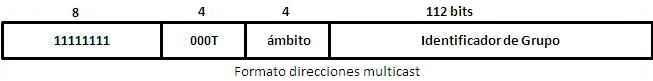
\includegraphics[width=\textwidth]{img/IPv6_MULTI.jpg}
\end{figure}

Las direcciones multicast comienzan con el prefijo \textbf{FF::/8}.
%%
\subsubsection{Direcciones públicas y privadas}
Las direcciones \textbf{Global Unicast} en IPv6 son el equivalente de las direcciones IP públicas en IPv4. Estas direcciones IP pueden ser encaminadas a través de la Internet. Actualmente usan el prefijo \textbf{2000::/3}, que permite $2^{45}$ sitios diferentes.\\


De igual modo que IPv4 dispone de direcciones \textbf{reservadas} para uso privado \textit{(Por ejemplo 192.168.x.x)}, IPv6 dispone de \textbf{ULA (Unique Local Addresses)}, que son todas las direcciones que comienzan con el prefijo \textbf{fc00::/7}.
%%
\subsubsection{Ámbitos y zonas}
Las direcciones IPv6 incluyen un \textbf{ámbito}, que indican en qué parte de la red la dirección es \textbf{válida}.\\

Una \textbf{zona} es una región conectada de la red de un ámbito determinado, dentro de la cual se garantiza que todas las direcciones son \textbf{únicas}. Dentro de una zona, los datagramas no se redirigen a una zona distinta, aunque sea del mismo ámbito. Para indicar la zona de una dirección se usa el símbolo \enquote{\%}.
\begin{center}
    \textit{Ejemplo: }FE80::1234\%1
\end{center}
\end{onepage}

%%%%%%%%%%%%%%%%%%%%%%%%
\subsection{Datagrama IPv6}
Un datagrama IPv6 está compuesto principalmente de dos partes: la cabecera y los datos.
\subsubsection{Cabecera}
\begin{figure}[H]
    \centering 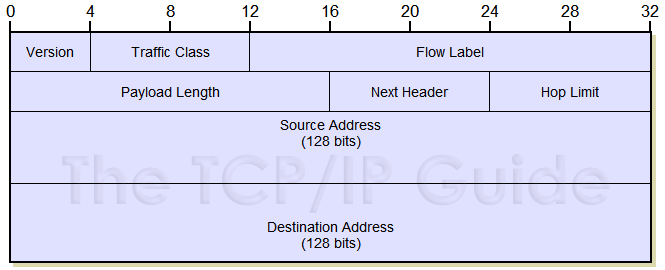
\includegraphics[width=0.8\textwidth]{img/ipv6_HEADER.png}
\end{figure}
\begin{itemize}
    \item \textbf{Traffic Class: }distingue diferentes requisitos de entrega del datagrama,es similar al campo DS/ToS de IPv4.
    \item \textbf{Flow Label: }Etiqueta el paquete como perteneciente a un \textbf{flujo} para mejorar el procesamiento realizado por los encaminadores de la red. Un flujo es un conjunto de paquetes que comparte las mismas características (origen/destino, requisitos, etc...).
    \item \textbf{Payload Length: }longitud sin contar la cabecera (máx. 64 Kbytes).
    \item \textbf{Hop Limit: }similar al campo TTL de IPv4.
    \item \textbf{Next Header: }Define la siguiente cabecera en el datagrama (dentro de la sección de datos), puede ser: 
    \begin{itemize}
        \item Una cabecera de extensión, similar al campo opciones de IPv4.
        \item un protocolo de nivel superior, encapsulado en la sección de datos (2=ICMP, 6=TCP, 17=UDP...)
    \end{itemize}
    \begin{figure}[H]
    \centering 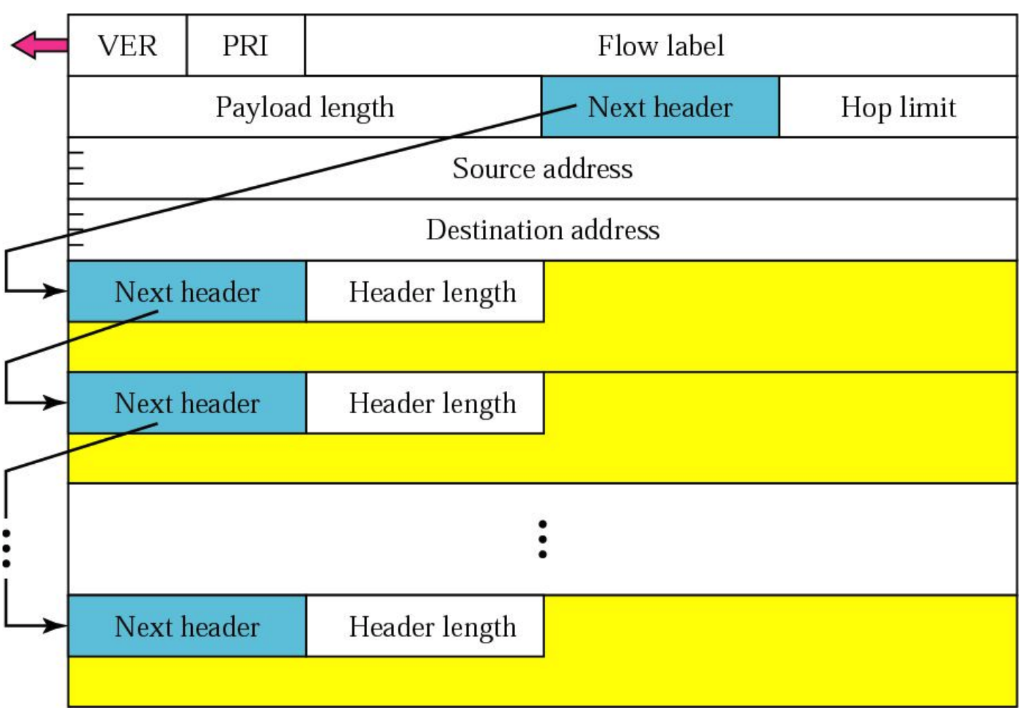
\includegraphics[width=0.6\textwidth]{img/IPv6_nextHeader.png}
\end{figure}
\end{itemize}

%%
\begin{onepage}
\subsubsection{Cambios con respecto a IPv6}
\begin{itemize}
    \item El campo Header Length se ha eliminado, ya que la longitud es fija.
    \item No hay campo Checksum, ya que se realiza por los protocolos superiores.
    \item Los campos de fragmentación se eliminan de la cabecera y se implementan en cabeceras de extensión.
\end{itemize}
%%
\subsubsection{Fragmentación}
Los routers IPv6 no hacen fragmentación. Los nodos IPv6 requieren ya sea hacer descubrimiento de MTU, realizar fragmentación extremo a extremo o enviar paquetes del tamaño mínimo MTU para IPv6 (1280 bytes).\\

\begin{figure}[H]
    \centering 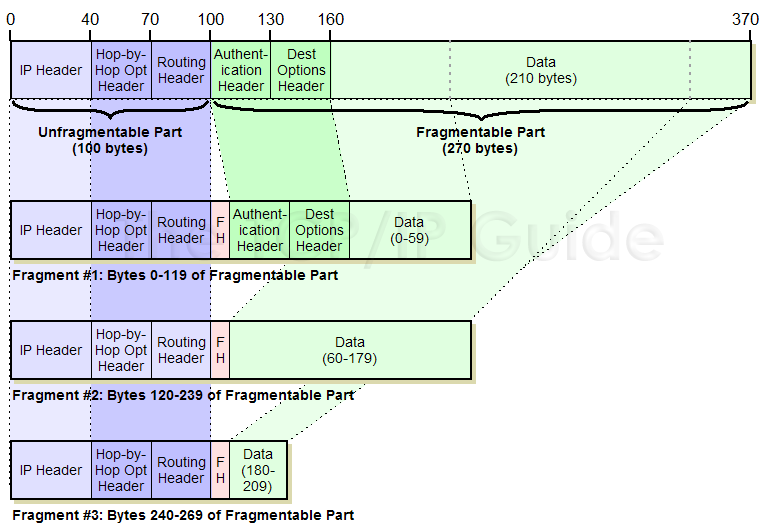
\includegraphics[width=\textwidth]{img/ipv6_fragm.png}
\end{figure}
\end{onepage}
%%%%%%%%%%%%%%%%%%%%%%%%%%%%%%%%%%%%%%%%%%%%%%%%%%
\section{Protocolo ICMPv6}
\begin{figure}[H]
    \centering 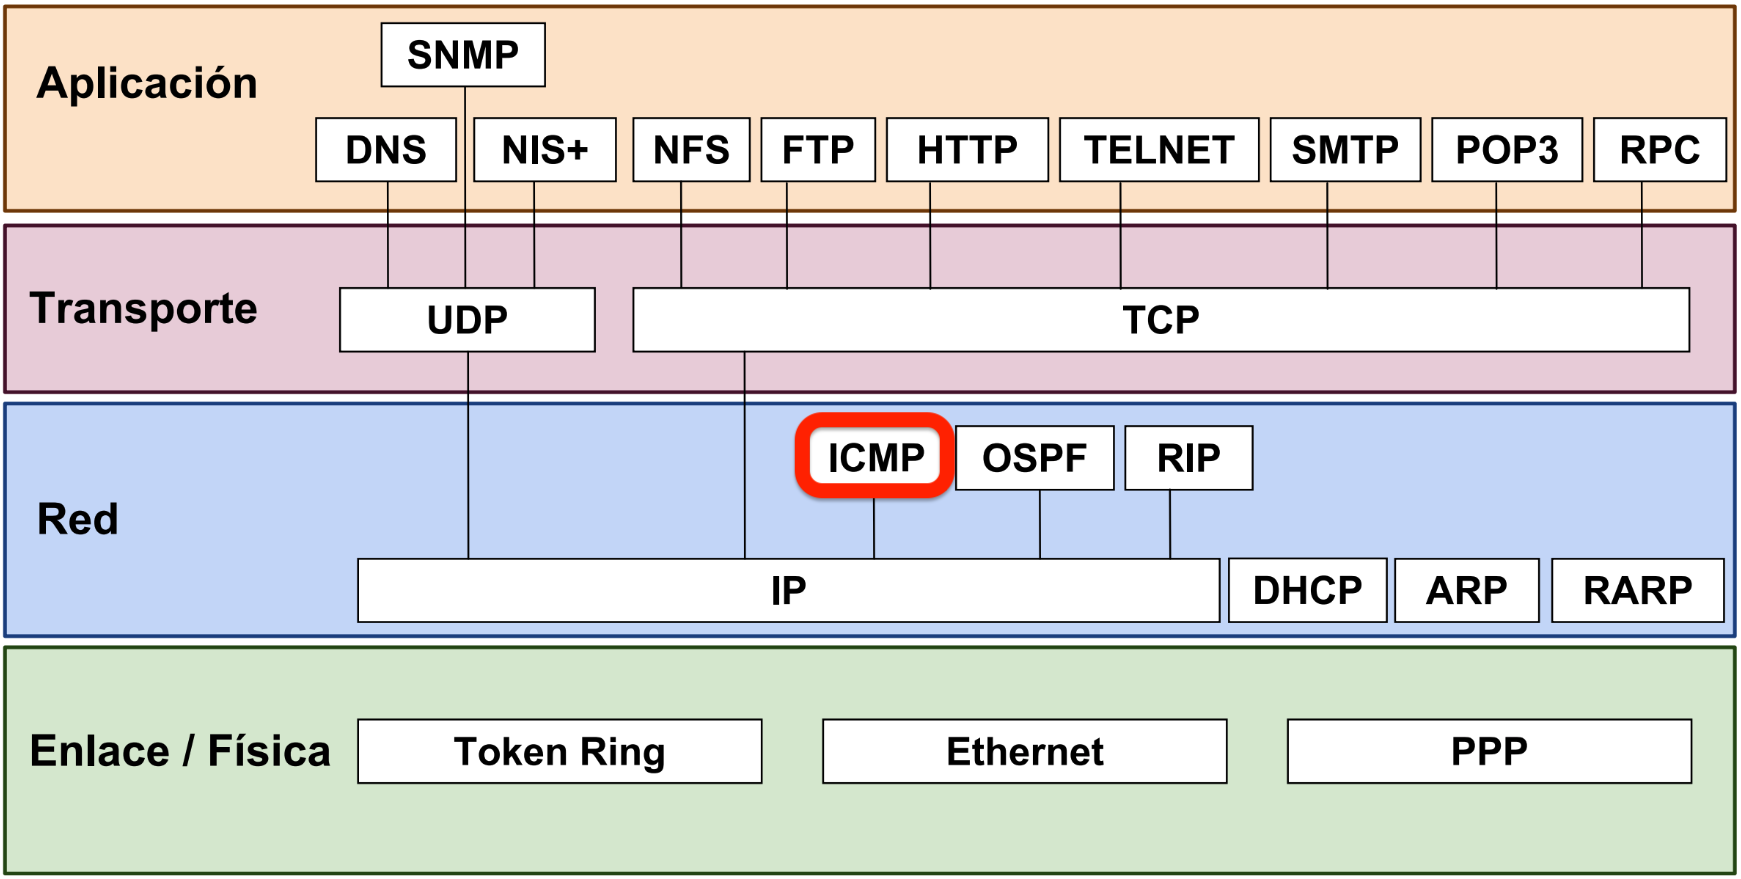
\includegraphics[width=0.7\textwidth]{img/ICMP.png}
\end{figure}
ICMPv6 (Internet Control Message Protocol version 6) es una nueva versión de ICMP y una parte importante de la arquitectura IPv6.\\

ICMPv6 asume el papel de los siguientes protocolos auxiliares en IPv4:
\begin{itemize}
    \item ICMPv4, protocolo de mensajes de control.
    \item IGMP, protocolo de gestión de grupos multicast.
    \item ARP, protocolo de resolución de direcciones.
\end{itemize}
Todos los mensajes ICMPv6 tienen un formato común:
\begin{figure}[H]
    \centering 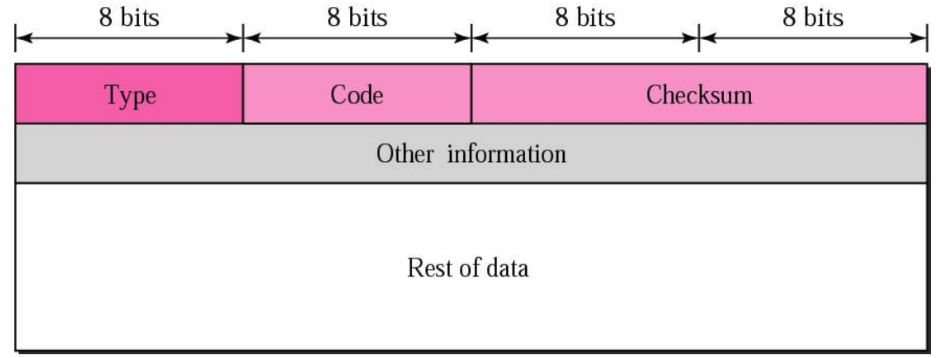
\includegraphics[width=0.7\textwidth]{img/ICMPv6_format.png}
\end{figure}
%%%%%%%%%%%%%%%%%%
\subsection{Mensajes ICMPv6}
%%%
\subsubsection{Mensajes de error}
Los mensajes de error se pueden producir cuando:
\begin{itemize}
    \item El destino es inalcanzable.
    \item El datagrama es demasiado grande.
    \item Tiempo excedido.
    \item Problema de parámetros.
\end{itemize}
\begin{onepage}
%%%
\subsubsection{Mensajes de información}
Proporcionan información de diagnóstico, pueden ser:
\begin{itemize}
    \item Echo request.
    \item Echo reply.
\end{itemize}
%%%
\subsubsection{Descubrimiento de vecinos}
\textbf{Neighbor Discovery (ND)} es un tipo de mensaje equivalente al protocolo Address Resolution Protocol (ARP) en IPv4.\\

Permite que los terminales aprendan las direcciones IPv6 de los vecinos y opera sobre hosts y routers en el mismo enlace.\\

Se pueden realizar las siguientes funciones:
\begin{itemize}
    \item \textbf{Descubrimiento de vecino.} Se utilizan dos tipos de mensajes:
    \begin{enumerate}
        \item Neighbor Solicitation.
        Este mensaje se genera para:
        \begin{itemize}
            \item Averiguar la dirección física asociada a una dirección IP (como ARP request en IPv4).
            \item Determinar si un nodo vecino sigue siendo alcanzable.
            \item Detectar si la dirección IP está duplicada.
        \end{itemize}
        \item Neighbor Advertisement.
        Este mensaje se genera para:
        \begin{itemize}
            \item Responder a un mensaje de solicitud de vecino (como ARP reply en IPv4).
            \item Anunciar un cambio en la dirección física de un interfaz.
        \end{itemize}
    \end{enumerate}
    \item \textbf{Descubrimiento de router.} Se utilizan dos tipos de mensajes:
    \begin{enumerate}
        \item Router Solicitation: este mensaje se genera tras la activación de un interfaz, para detectar los encaminadores y realizar la autoconfiguración del interfaz.
        \item Router Advertisement: los envían los routers para anunciar su presencia en la red. Son enviados de forma periódica y como respuesta a mensajes Router Solicitation.
    \end{enumerate}
    \item \textbf{Redirección.} Permite notificar a un host una ruta más adecuada para alcanzar un determinado destino.
\end{itemize}
\end{onepage}
%%%%%%%%%%%%%%%%%%%%%%%%%%%%%%%%%%%%%%%%%%%%%%%%%%
\section{Encaminamiento en Internet}
En una red, el encaminamiento consiste en encontrar un camino, desde el origen al destino, a través de nodos de conmutación o routers intermedios. También es necesario decidir cuál es el mejor camino posible (camino más corto) según alguna métrica \textit{(número de nodos, distancia geográfica, retardo, etc...)}.\\

Cuando un encaminador recibe un paquete lo retransmite por el enlace
adecuado para alcanzar el destino. Esta elección la realiza según:

\begin{itemize}
    \item \textbf{Tablas de encaminamiento.} Guardan una lista de las direcciones IP y el siguiente salto que tienen asociado.
    \item \textbf{Etiquetas.} Cada datagrama IP se etiqueta y se conmuta según una etiqueta (campo \enquote{Flow Label} en IPv6). Esto reduce la complejidad de la tabla de encaminamiento.
\end{itemize}
%%%%%%%%%%%%%%%%%%%%%%
\subsection{Técnicas de Encaminamiento}
\begin{itemize}
    \item \textbf{Encaminamiento local: } no tiene en cuenta la topología de la red y usa únicamente información local. Las técnicas más comunes son: Encaminamiento aleatorio, Encaminamiento aislado, e Inundación.
    \item \textbf{Encaminamiento estático: }Las tablas de encaminamiento se construyen manualmente y no se adaptan a los cambios de la red.
    \item \textbf{Encaminamiento dinámico: }las tablas de encaminamiento se construyen de forma automática, mediante el intercambio periódico de información entre los encaminadores. Las técnicas más comunes son:
    \begin{itemize}
        \item Encaminamiento por \textbf{vector de distancias} \textit{(ejemplo: RIP)}.
        \item Encaminamiento por \textbf{estado de los enlaces} \textit{(ejemplo: OSPF)}.
        \item Encaminamiento por \textbf{vector de rutas} \textit{(ejemplo: BGP)}.
    \end{itemize}
    \end{itemize}
    \begin{tcolorbox}[
    title=Sistemas Autónomos (AS),
    colback=blue!5!white,
    colframe=blue!75!black,
    fonttitle=\bfseries]
    Un AS es una conjunto de redes y encaminadores gestionados y administrados por una misma autoridad. Se componen de:
    \begin{itemize}
        \item \textbf{Routers Internos: }interconectan redes dentro del propio AS. Utilizan \textbf{protocolos internos (IGP)} como RIP o OSPF.
        \item \textbf{Routers Frontera: }interconectan varios ASs. Utilizan \textbf{protocolos externos (EGP)} como BGP.
    \end{itemize}
    \end{tcolorbox}
\begin{onepage}
    %%%%%%%%%%%%%%%%%%%%%%%%%%%%%%%%%%%%%%%%%%%%%%%%
    \section{Vector de distancias - Protocolo RIP}
    El \textbf{vector de distancias} es un método de enrutamiento que utiliza el algoritmo de Bellman-Ford para calcular las rutas.
    %%%%%%%%%%%%%%%%%%%%%%
    \subsection{Funcionamiento}
    Imaginemos una red con la siguiente topología:
    \begin{figure}[H]
    \centering 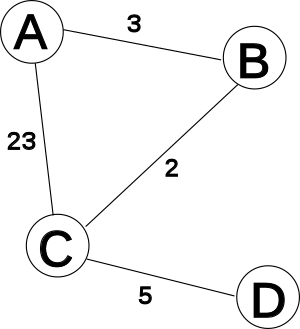
\includegraphics[width=0.2\textwidth]{img/VectorDeDistanciasEj1.png}
    \caption{Consta de 4 nodos. El número encima de cada arista indica la distancia del enlace.}
    \end{figure}
    Inicialmente los routers sólo conocen sus rutas directas. Vemos como en cuatro unidades de tiempo (T), todos los routers disponen de todas las distancias posibles.
    \begin{figure}[H]
    \centering 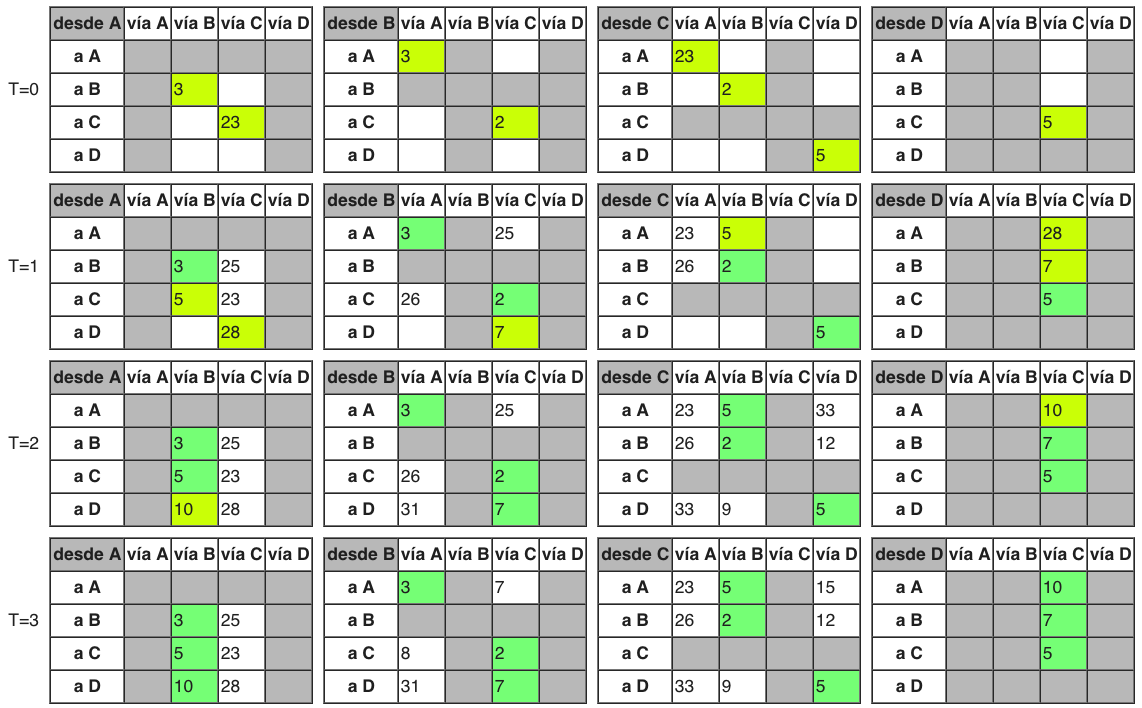
\includegraphics[width=1.1\textwidth]{img/VectorDeDistanciasEj2.png}
    \caption{El camino más corto está marcado con el color verde, un camino más corto nuevo está indicado en amarillo.}
    \end{figure}
    \end{onepage}
    
    \begin{onepage}
    %%%%%%%%%%%%%%%%%%%%%%
    \subsection{Problemas}
     El algoritmo Bellman-Ford utilizado en Vector de Distancias no previene de la aparición de bucles. El problema de la \textbf{cuenta a infinito} es que hace que los costes o distancias se incrementen indefinidamente sin que el algoritmo llegue a converger nunca.
    \begin{figure}[H]
    \centering 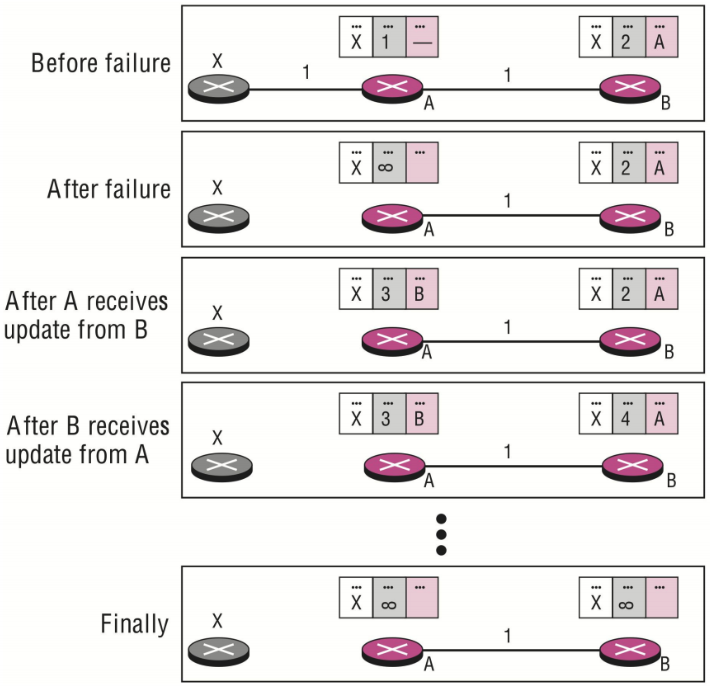
\includegraphics[width=0.7\textwidth]{img/CuentaAInfinito.png}
    \end{figure}
    \textbf{Soluciones} a la cuenta a infinito:
    \begin{itemize}
        \item \textbf{Establecer el infinito a un número pequeño. }\textit{Por ejemplo, en RIP el infinito se establece en 16 saltos.}
        \item \textbf{Horizonte dividido: }los destinos aprendidos a través de un determinado enlace nunca se difunden a través de dicho enlace. \textit{Ejemplo: El nodo B no enviará al nodo A información sobre el destino X.}
        \item \textbf{Horizonte dividido con ruta inversa envenenada: }los destinos aprendidos a través de un determinado enlace sí se difunden a través de dicho enlace, pero con distancia infinita. \textit{Ejemplo: El nodo B anunciará al nodo A que el destino X está a distancia infinita.}
        \item \textbf{Actualizaciones forzadas: }cuando un encaminador detecta una modificación en su tabla de rutas inmediatamente difunde esta información a sus vecinos. De esta forma, los cambios en la topología se propagan de forma rápida a todos los puntos de la red.
    \end{itemize}
\end{onepage} 

\begin{onepage}
    %%%%%%%%%%%%%%%%%%%%%%
    \subsection{Protocolo RIP}
    \begin{figure}[H]
    \centering 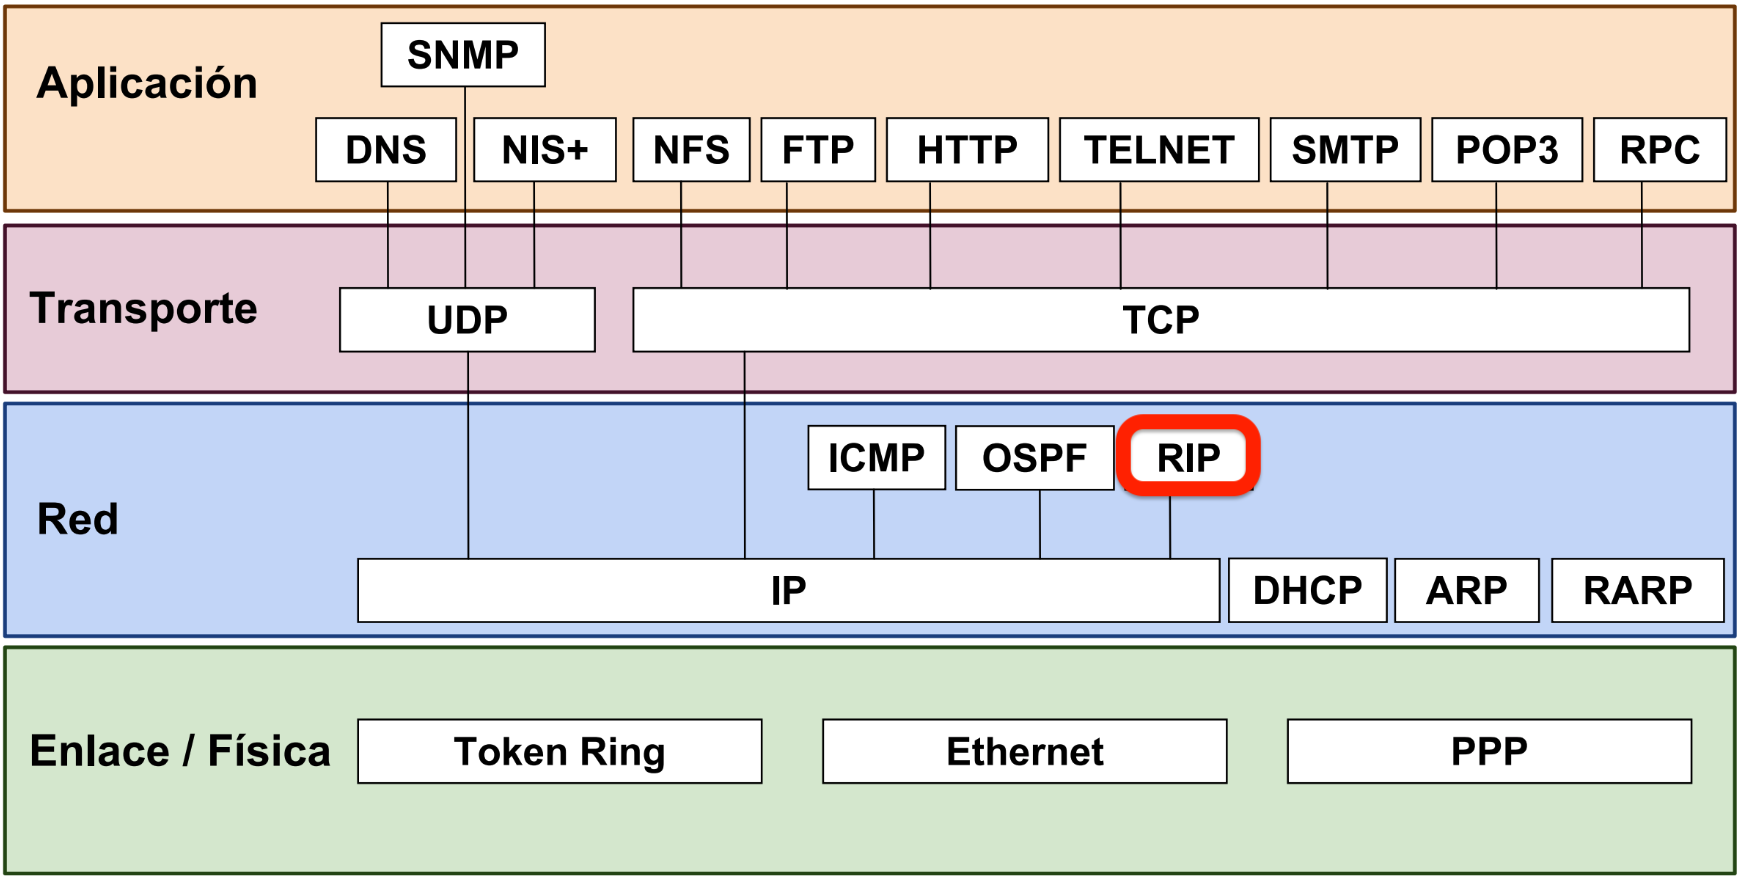
\includegraphics[width=0.7\textwidth]{img/RIP.png}
    \end{figure}
    
    RIP (Routing Information Protocol), es un protocolo de puerta de enlace interna (Interior Gateway Protocol, IGP) utilizado por los routers para intercambiar información acerca de redes IP. Su algoritmo de encaminamiento está basado en el \textbf{vector de distancia}, ya que calcula la ruta más corta posible a partir del número de saltos.\\
    
    %%%%%
    \subsubsection{Versiones}
    \begin{itemize}
        \item RIP versión 1 (1993).
        \item RIP versión 2 (1998).
        \item RIPng para IPv6 (1997).
    \end{itemize}
    %%%%%
    \subsubsection{Mensajes}
    Los mensajes tienen una cabecera con el tipo de mensaje y la versión del protocolo RIP, y un máximo de 25 entradas.\\
    
    Las entradas en \textbf{RIPv1} contienen la dirección IP de la red de destino y la métrica. Las entradas en \textbf{RIPv2} incluyen además su máscara y el siguiente encaminador.\\
    
    Los mensajes RIP pueden ser de dos tipos:
    \begin{itemize}
        \item \textbf{Petición (REQUEST): }enviados por algún encaminador recientemente iniciado que solicita información de los encaminadores vecinos.
        \item \textbf{Respuesta: (RESPONSE)}mensajes con la actualización de las tablas de encaminamiento. Existen tres tipos:
        \begin{enumerate}
            \item Periódicos: Se envían cada 30 segundos. Para indicar que el enlace y la ruta siguen activos. Se envía la tabla de encaminado completa.
            \item Mensajes enviados como respuesta a mensajes de petición.
            \item Mensajes enviados cuando cambia algún coste. Se envía toda la tabla de encaminado.
        \end{enumerate}
    \end{itemize}
    \end{onepage}
    %%%%%%
    \subsubsection{Temporizadores}
    RIP utiliza distintos temporizadores:
    \begin{itemize}
        \item \textbf{Temporizador periódico: }controla la publicación de los mensajes periódicos. Se debe ajustar el temporizador a 30s.
        \item \textbf{Temporizador de caducidad: }establece cuanto tiempo puede estar una ruta en la tabla sin ser actualizada.
        \item \textbf{Temporizador de Recolección de Basura: }controla el tiempo que pasa entre que una ruta es invalidada (o marcada como inalcanzable) y el tiempo que pasa hasta que se elimina la entrada de la tabla de ruteo.
    \end{itemize}

\begin{onepage}
    %%%%%%%%%%%%%%%%%%%%%%%%%%%%%%%%%%%%%%%%%%%%%%%%
    \section{Estado de los enlaces - Protocolo OSPF}
    \textbf{Estado de los enlaces} consiste en que un router comunica al resto de nodos de la red cuáles son sus vecinos y a qué distancia está de ellos. Con la información que un nodo de la red recibe de todos los demás, puede construir un \enquote{mapa} de la red, y sobre él calcular los caminos óptimos. El encaminamiento por estado de enlace sustituyó al método de vector de distancias.\\
    
    \textbf{Funcionamiento.} Lo podemos dividir en cinco pasos fundamentales:
    \begin{enumerate}
        \item Descubrir a sus vecinos y sus direcciones.
        \item Medir el costo a cada uno de sus vecinos.
        \item Construir el paquete con la información recabada.
        \item Enviar este paquete al resto de routers.
        \item Calcular la ruta mínima al resto de routers. Una vez que el router ha completado la recopilación de información, puede construir el grafo de la subred. De esta manera, se puede utilizar el algoritmo de Dijkstra para calcular el camino más corto a todos los nodos.
    \end{enumerate}
    %%%%%%%%%%%%%%%%%%%%%%%%%%
    \subsection{Protocolo OSPF}
    \begin{figure}[H]
    \centering 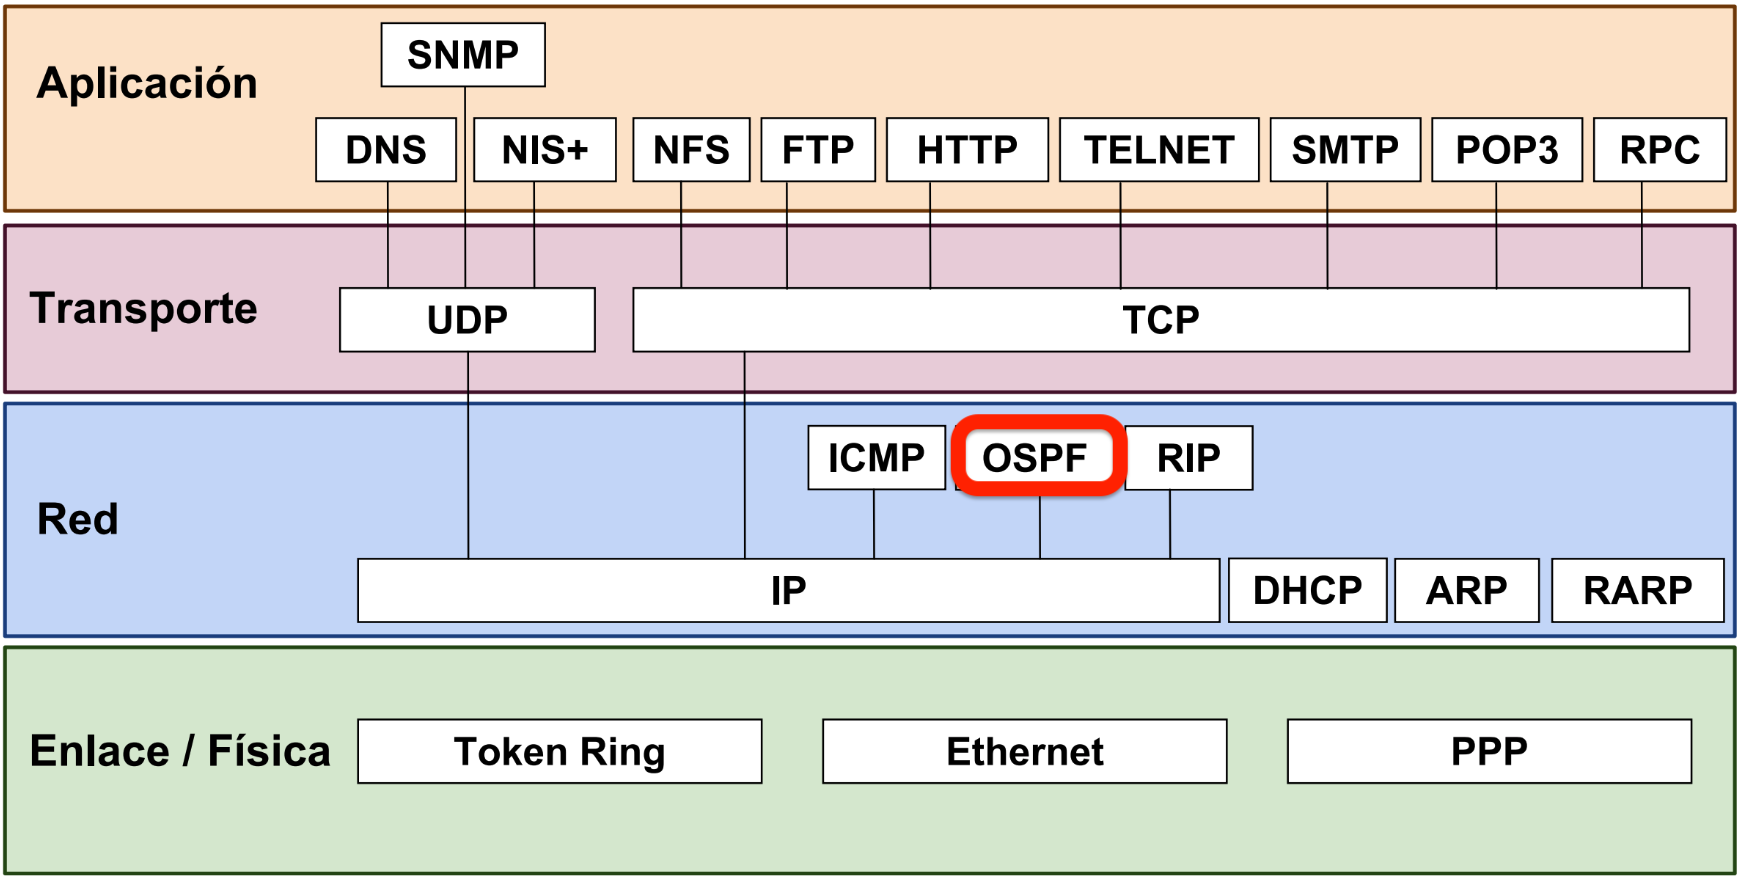
\includegraphics[width=0.7\textwidth]{img/OSPF.png}
    \end{figure}
    \textbf{OSPF (Open Shortest Path First)}, es un protocolo de red para encaminamiento jerárquico de pasarela interior (IGP), que usa el algoritmo Dijkstra para calcular la ruta más corta entre dos nodos.\\
    
    Su medida de métrica se denomina \textbf{cost}, y tiene en cuenta diversos parámetros tales como el ancho de banda y la congestión de los enlaces. OSPF es probablemente el protocolo IGP más utilizado en redes grandes.
\end{onepage}
\begin{onepage}
    Se desarrolló como alternativa a RIP para aliviar sus limitaciones:
    \begin{itemize}
        \item Distribuye la carga entre caminos equivalentes.
        \item Particionado lógico de la red para reducir la cantidad de información anunciada.
        \item Convergencia más rápida, propaga inmediatamente los cambios en las rutas.
        \item Soporte para máscaras de longitud variable (VLSM) y CIDR
    \end{itemize}
    \begin{tcolorbox}[
    title=Área,
    colback=blue!5!white,
    colframe=blue!75!black,
    fonttitle=\bfseries]
    Es una agrupación lógica de encaminadores y redes, con un identificador de área de 32 bits (Area ID).\\
    
    Los encaminadores mantienen únicamente información de su área y limitan el número de intercambios de información de los enlaces.
    \end{tcolorbox}
    %%%%%%%%
    \subsubsection{Tipos de router en OSPF}
    \begin{itemize}
    \item \textbf{Intra-Area Routers (IA): }todos sus interfaces están en el área y mantiene sólo información de la topología de su área.
    \item \textbf{Area Border Routers (ABR): }conectado a dos o más áreas. Mantiene una Base de Datos para cada una de las áreas a las que está conectado.
    \item \textbf{AS Boundary Routers (ASBR): } Situado en la frontera del AS, intercambia rutas entre la red OSPF y otros sistemas.
    \end{itemize}
    %%%%%
    \subsubsection{Relación con los vecinos en OSPF}
    Cada router OSPF realiza un seguimiento de sus nodos vecinos. Para el descubrimiento de vecinos se utiliza el protocolo \textbf{OSPF Hello}.\\
    
    OSPF utiliza paquetes \textbf{hello} y dos temporizadores para saber si un vecino sigue disponible. Cuando un router recibe un mensaje Hello de otro router que contiene su propio ID, establece una relación de vecindad con dicho router.\\
    
    Después de establecer la vecindad se intercambian las base de datos con el
    estado de los enlaces. Con esa información construye su árbol de rutas. El árbol de rutas incluye tanto encaminadores (ID) como redes (IP) y el coste
    asociado.
\end{onepage}

%%%%%%%%%%%%%%%%%%%%%%%%%%%%%%%%%%%%%%%%%%%%%%%%
\section{Vector de Rutas - Protocolo BGP}
\textbf{Vector de Rutas} es un protocolo de enrutamiento de red que mantiene la información de ruta actualizada dinámicamente. Está basado en el de vector de distancias.\\

Es diferente del enrutamiento por vector de distancia y el enrutamiento por estado de enlace. Cada entrada en la tabla de enrutamiento contiene la red de destino, el siguiente router y la ruta para llegar al destino. Utiliza CIDR y detecta bucles de forma sencilla.
%%%%%%%%%%%%%%%%%%%%%%%
\subsection{Protocolo BGP}
\textbf{BGP (Border Gateway Protocol)} es un protocolo de intercambio de información de encaminamiento entre sistemas autónomos. Es un ejemplo de protocolo \textbf{EGP}.\\

Los encaminadores intercambian la tabla de rutas cuando establecen la conexión inicial y periódicamente se envían actualizaciones incrementales de la tabla inicial.
%%%%%
\subsubsection{Mensajes BGP}
\begin{itemize}
    \item \textbf{OPEN: }Establece la sesión BGP. Incluye identificador de AS y parámetros de configuración.
    \item \textbf{UPDATE: }Actualización incremental de la información de encaminamiento. Cada mensaje puede incluir una red alcanzable en CIDR con sus atributos, incluida la ruta, y una lista de redes retiradas.
    \item \textbf{NOTIFICATION: }Se envía a los vecinos cuando se detecta un error. Implica un cierre de la sesión y la invalidación de las rutas asociadas.
    \item \textbf{KEEPALIVE: }Para asegurar que la sesión permanezca activa. Se envía en respuesta a un mensaje OPEN y periódicamente para informar de la
    presencia del encaminador. Si pasado un tiempo (hold) no se recibe información, se cierra la sesión.
\end{itemize}